%\documentclass[11pt]{report}



%\begin{document}

\chapter{Private phylogenetic trees}
\label{ch:phylogenetic-trees}

Several privacy-enhancing technologies (PET) (differential privacy \cite{Li2016}, homomorphic encryption \cite{Armknecht2015} and secure multiparty computation) have already been applied to biomedical data analysis \cite{Verhaert2018, Scardapane2017, Maulany2018, Kikuchi2018, Tawfik2018}. In particular, these classical techniques have been used in the context of genomic private data analysis. As a way to push research and innovation forward, there have been several competitions \cite{Wang2017} focused on developing faster and more secure solutions in the field of genomic analysis. Also, in recent surveys \cite{MY19, Naveed2015}, the authors describe the role of PETs in four different computational domains of the genomic's field (genomic aggregation, GWASs and statistical analysis, sequence comparison and genetic testing). However, these surveys do not provide any reference covering privacy-preserving methods applied to phylogeny inference. 

In contrast to classical technologies, the usage of quantum cryptographic technologies in private computation has not been widely reported. Chan et al. \cite{Chan2014} developed real-world private database queries assisted with quantum technologies and in \cite{Ito2017} the authors simply suggest that their implementation of quantum OT is suitable to be applied in an SMC environment. %In \cite{Pinto2020}, it is presented a system assisted with quantum technologies for the private recognition of composite signals in genome and proteins and in \cite{SGPM21} the authors give a brief description of a private UPGMA (Unweighted Pair Group Method with Arithmetic mean) protocol assisted with quantum technologies. 
Despite its little integration with PETs, quantum cryptographic technologies have already reached a maturity level that enables this integration. Quantum key distribution (QKD) and quantum random number generators (QRNG) are currently being commercialized and applied to critical use cases (e.g. Governmental data storage and communications, Data centres \cite{AM19}) with in-field deployment (e.g. OpenQKD, https://openqkd.eu/). The quantum oblivious key distribution (QOKD) protocol is based on the same technology as QKD and QRNG, benefiting from its development and allowing to generate the necessary resources to execute OT \cite{Lemus20, JSGBBWZ11, KWW12}. 

%Furthermore, only SMC classical frameworks have been applied to the private analysis of genomic data. In a recent survey \cite{MY19}, the authors describe the role of privacy enhancing techniques (Differential Privacy, Homomorphic Encryption and SMC) in four different computational domains (genomic aggregation, GWASs and statistical analysis, sequence comparison and genetic testing). However, to the best of our knowledge, there is no tailored protocol to the computation of phylogentic trees. 

%Here we propose and demonstrate the feasibility of aSecure  Multiparty  Computation  (SMC)  system  assisted  with  quantum  communication  technologies  thatis  designed  to  compute  a  phylogenetic  tree  for  a  set  of  genome  sequences.  This  system  significantlyimproves  the  privacy  and  security  of  the  computation  thanks  to  three  quantum  cryptographic  protocolsthat  provide  security  against  quantum  computer  attacks.  Also,  it  decreases  the  complexity  of  the  actual computation when compared to a purely classical system. 

In this chapter, we present a feasible modular private phylogenetic tree protocol that leverages quantum communications. It provides enhanced security against quantum computer attacks and decreases the complexity of the computation phase when compared to a state-of-the-art classical-only system. 
%We present a feasible modular protocol for privately computing phylogenetic trees that is secure against quantum computer attacks and do not add any efficiency overhead during the execution phase. 
The system is built on top of Libscapi \cite{libscapi} implementation of Yao protocol and PHYLIP phylogeny package \cite{PH78}. It integrates three crucial quantum primitives: quantum oblivious transfer, quantum key distribution and quantum random number generator.

This chapter follows a top-down approach. In section \ref{phyloTree}, we start by explaining the concept of phylogenetic trees and the distance-based algorithms used to generate these trees. In section \ref{secDefition}, we set down the security definitions that will be used to analyse and prove the system's security. %In section \ref{cryptoTools}, we explain the cryptographic tools used in the system. 
In sections \ref{quantumTools} and \ref{softTools}, we describe the quantum cryptographic tools and the software tools that are integrated into the protocol, respectively. In section \ref{smcPhylo}, we describe the proposed SMC system for phylogenetic trees. In section \ref{quantumTechIntegration} we explain how the quantum cryptographic tools are integrated into the system. Section \ref{systemSecurity} is devoted to the theoretical security analysis of the protocol and in section \ref{CompleAnalysis} we perform a complexity analysis. In the last section we present a performance comparison of the system between a classical-only and a quantum-assisted implementation.



\section{Phylogenetic trees} \label{phyloTree}

%Phylogenetic trees are commonly compared with family trees in the following sense. The same way as family trees represent the historical ties of blood, phylogenetic trees represent the historical ties of genes. Thus, p
Phylogenetic trees are diagrams that depict the evolutionary ties between groups of organisms \cite{M10} and are composed of several nodes and branches. The nodes represent genome sequences and each branch connects two nodes. It is important to note that the terminal nodes (also called leaves) represent known data sequences, whether internal nodes are ancestral sequences inferred from the known sequences \cite{Z06, Felsenstein2003}. The length of the branches connecting two nodes represents the number of substitutions that have occurred between them. However, this quantity must be estimated because it cannot be computed directly using the sequences. In fact, by simply counting the number of sites where two nodes have different base elements (Hamming distance), we underestimate the number of substitutions that have occurred between them. 

The best way to compute a correct phylogenetic tree depends on the type of species and sequences under analysis and the assumptions made by the sequences substitution model. By a correct tree, we mean a tree that depicts as approximate as possible the real phylogeny of the sequences, i.e. the real ties between known sequences and inferred ancestors. These assumptions lead to different algorithms which can be divided into two categories:

\begin{enumerate}
    \item Distance-based methods: they base their analysis on the evolutionary distance matrix which contains the evolutionary distances between every pair of sequences. The evolutionary distance used also depends on the substitution model considered. These methods are computationally less expensive when compared to character-based methods.
    \item Character-based methods: they base their analysis on comparing every site (character) of the known data sequences and do not reduce the comparison of sequences to a single value (evolutionary distance). 
\end{enumerate}

We only consider the distance-based algorithms that are part of the PHYLIP \cite{F89} distance matrix models, namely: Fitch-Margoliash (\texttt{fitch} and \texttt{kitsch}), Neighbour Joining  (\texttt{neighbor}) and UPGMA (\texttt{neighbor}). Also, we only consider the evolutionary distances developed in PHYLIP \texttt{dnadist} program:  Jukes-Cantor (JC) \cite{JC69}, Kimura 2-parameter (K2P) \cite{K80}, F84 \cite{F84} and LogDet \cite{L94}. We refer interested readers on this topic to some textbooks about phylogenetic analysis \cite{Z06, Felsenstein2003}. %[Yang, Z. (2006).	Computational molecular evolution. Oxford University Pres, Felsenstein,	J.	(2004). Inferring phylogenies and Phylogenetic Inference, chpt 11 Swofford].

Next, we give an overview of these distance-based methods to build some intuition on how to tailor them to a private setting. We start by looking at the different evolutionary distances and then at the distance-based algorithms.

\subsection{Evolutionary distances} \label{evolDist}

The evolutionary distance depends on the number of estimated substitutions between two sequences, which is governed by the substitution model used. So, before defining a suitable distance, it is important to have a model that describes the substitution probability of each nucleotide across the sequence at a given time. 

The distances considered in this work can be divided into two groups by their assumptions. JC, K2P and F84 assume that the substitution probabilities remain constant throughout the tree, (i.e. stationary probabilities), whether the LogDet distance assumes that the probabilities are not stationary.  

%"Since the genetic distance cannot be observed directly, statistical techniques are necessary to infer this quantity from the data".


%These must be additive in the sense that the distance between sequence $x$ and sequence $z$ with intermediate sequence $y$ must be given by the additive formula below:

%$$d_{xz} = d_{xy} + d_{yz}$$

%So, before computing phylogenetic trees with this property, we have to estimate the evolutionary distance first. In order to do so, it is important to have a model that describes the substitution probability of each nucleotide across the sequences at a given time. The four distances considered in this work falls into two types of assumptions: LogDet distance assumes that the substitution probabilities may not remain constant throughout the tree and the other three distances (JC, K2P and F84) assume stationary probabilities.

Also, the first three evolutionary distances (JC, K2P and F84) assume an evolutionary model that can be described by a \textit{time-homogeneous stationary Markov} process. %This reflects the fact that these models have the following assumptions: %\begin{enumerate}
%    \item All the nucleotide replacements are random and independent of each other;
%    \item The nucleotide frequencies present in the data do not change over time and from sequence to sequence.
%\end{enumerate} 
This Markov process is based on a probability matrix $\mathbf{P}(t)$ that defines the transition probabilities from one state to the other after a certain time period $t$. It can be shown \cite{PM09} %check references [https://www2.ib.unicamp.br/profs/sfreis/SistematicaMolecular/Aula06SelecaoModelosSubstituicaoI/Leituras/The%20Phylogenetic%20Handbook%20-%20Chapter%204.pdf]
that this probability is given by 

\begin{equation}
\mathbf{P}(t) = e^{\mathbf{Q}t}
\label{eq:probability}
\end{equation}
where the rate matrix $\mathbf{Q}$ is of the form given by (\ref{eq:Qmatrix}).

%\begin{figure*}[h!]
% ensure that we have normalsize text
%\normalsize
%\begin{equation}
%    \mathbf{Q} = \begin{pmatrix}
%-\mu(a\pi_C+b\pi_G + c\pi_T) & a\mu\pi_C & b\mu\pi_G & c\mu\pi_T\\
%g\mu\pi_A&-\mu(g\pi_A+d\pi_G + c\pi_T) & d\mu\pi_G & e\mu\pi_T\\
%h\mu\pi_A & i\mu\pi_C & -\mu(h\pi_A+j\pi_C + f\pi_T) & f\mu\pi_T\\
%j\mu\pi_A & k\mu\pi_C & l\mu\pi_G & -\mu(i\pi_A+k\pi_C + l\pi_G)
%\end{pmatrix}
%\label{eq:Qmatrix}
%\end{equation}
% The spacer can be tweaked to stop underfull vboxes.
%\vspace*{4pt}
%\end{figure*}

\begin{footnotesize}
\begin{equation}
\mathbf{Q} = \begin{pmatrix}
-\mu(a\pi_C+b\pi_G + c\pi_T) & a\mu\pi_C & b\mu\pi_G & c\mu\pi_T\\
g\mu\pi_A&-\mu(g\pi_A+d\pi_G + c\pi_T) & d\mu\pi_G & e\mu\pi_T\\
h\mu\pi_A & i\mu\pi_C & -\mu(h\pi_A+j\pi_C + f\pi_T) & f\mu\pi_T\\
j\mu\pi_A & k\mu\pi_C & l\mu\pi_G & -\mu(i\pi_A+k\pi_C + l\pi_G)
\end{pmatrix}
\label{eq:Qmatrix}
\end{equation}
\end{footnotesize}


In $\mathbf{Q}$, each entry $\mathbf{Q}_{ij}$ represents the substitution rate from nucleotide i to j and both its columns and rows follow the order $A$, $C$, $G$, $T$. $\mu$ is the total number of substitutions per unit time and we can define the evolutionary distance, $d$, to be given by $d = \mu t$. The parameters $a, b, c, ..., l$ represent the relative rate of each nucleotide substitution to any other. Finally, $\pi_A, \pi_C, \pi_G, \pi_T$ describe the frequency of each nucleotide in the sequences. 

From expression (\ref{eq:probability}), it is possible to define a likelihood function on the distance $d$ and use the maximum likelihood approach to get an estimation of the evolutionary distance. The likelihood function defines the probability of observing two particular sequences, $x$ and $y$, given the distance $d$:

$$L(d) = \prod_{i=1}^n \pi_{x_i}P_{x_i, y_i}\Big(\frac{d}{\mu}\Big)$$

The parameters of $\mathbf{Q}$ are defined differently depending on the evolutionary model used and the maximum likelihood solution leads to different evolutionary distances. 

\subsubsection{Jukes-Cantor}\label{JK_model}

The Jukes-Cantor model \cite{JC69} is the simplest possible model based on $\mathbf{Q}$ as given in (\ref{eq:Qmatrix}). It assumes the frequencies of the nucleotide to be the same, i.e. $\pi_A = \pi_C = \pi_G = \pi_T = \frac{1}{4}$ and sets the relative rates $a=b= ... = l = 1$. This model renders an evolutionary distance between two sequences $x$ and $y$ given by:

\begin{equation}
d_{xy} = -\frac{3}{4}\ln \bigg(1- \frac{4}{3}\frac{h_{xy}}{n}\bigg)
\label{eq:JC_distance}
\end{equation}
where $h_{xy}$ is the uncorrected hamming distance and $n$ the length of the sequences.

\subsubsection{Kimura 2-parameter}\label{K2P_model}

This model \cite{K80} distinguishes between two different nucleotide mutations:

\begin{enumerate}
    \item Type I (transition): $A\leftrightarrow G$, i.e. from purine to purine, or $C\leftrightarrow T$, i.e. from pyrimidine to pyrimidine.
    \item Type II (transversion): from purine to pyrimidine or vice versa.
\end{enumerate}

These two different types of transformation lead to different probability distributions denoted by $P$ and $Q$, where P is the probability of homologous sites showing a type I difference, while Q is that of these sites showing a type II difference. So, the Kimura \cite{K80} metric between $x$ and $y$ is given by the following:

\begin{equation}
d_{xy} = -\frac{1}{2}\ln\bigg( \big(1-2P-Q\big) \sqrt{1-2Q} \bigg)
\end{equation}
where $P=\frac{n_1}{n}$, $Q=\frac{n_2}{n}$ and $n_1$ and $n_2$ are respectively the number of sites for which two sequences differ from each other with respect to type I ("transition" type) and type II ("transversion" type) substitutions.

\subsubsection{F84}\label{F84_model}

This model \cite{F84} also distinguishes different nucleotide transitions but do not assume the nucleotide frequencies to be the same. This leads to a more general distance which can be estimated in closed form:

\begin{equation}
    d_{xy} = -2 A\ln\left( 1- \frac{P}{2A} - \frac{(A-B)Q}{2AC} \right) + 2(A-B-C)\ln\bigg( 1-\frac{Q}{2C} \bigg)
\label{eq:F84_distance}
\end{equation}
where $A = \frac{\pi_C \pi_T}{\pi_Y} + \frac{\pi_A \pi_G}{\pi_R}$, $B=\pi_C\pi_T + \pi_A\pi_G$ and $C=\pi_R\pi_Y$ for $\pi_Y = \pi_C + \pi_T$ and $\pi_R = \pi_A + \pi_G$, and $P$ and $Q$ are defined as in the Kimura 2-parameter model above.

Although more complex models can be considered with different combinations of parameters in $\mathbf{Q}$, not all of them produce a distance function that can be estimated in closed form. 

\subsubsection{LogDet}\label{LD_model}

As mentioned before, the models based on matrix $\mathbf{Q}$ assume that the probability matrix $\mathbf{P}(t)$ is stationary, i.e. remains constant throughout the tree. However, there are evolutionary scenarios where this assumption does not give a correct description of reality. The LogDet evolutionary distance \cite{L94} suits a wider set of models and considers the case where $\mathbf{P}(t)$ is different at each branch in the tree. This is given by

\begin{equation}
    d_{xy} = -\frac{1}{4}\ln\Bigg( \frac{\det F_{xy}}{\sqrt{\det \prod_x \prod_y}} \Bigg)
\label{eq:LogDet_distance}
\end{equation}
where the divergence matrix $F_{xy}$ is a $4\times 4$ matrix such that the $ij-$th entry gives the proportion of sites with nucleotide $i$ in sequence $x$ and $j$ in sequence $y$. Also, $\prod_x$ and $\prod_y$ are diagonal matrices where its $i-$th component correspond to the proportion of $i$ nucleotide in the sequence $x$ and $y$, respectively.

\subsection{Distance-based algorithms}

All distance-based methods make use of evolutionary distances to compare different genomic sequences. Although it may lead to less accurate phylogenetic trees, these methods are highly popular among researchers who have to handle large number of sequences. All methods assume the following:

\begin{enumerate}
    \item The evolutionary distance computed between each pair is independent of all other sequences;
    \item The estimated distance between each pair of sequences is given by the sum of the size of the branches that connect both of them.
\end{enumerate}

These algorithms are thus divided into two phase: 

\begin{enumerate}
    \item Distance computation phase: all the pairwise evolutionary distances are computed according to the selected model. This step is common to all distance-based methods;
    \item Iterative clustering: aggregate the sequences in clusters iteratively. This step is specific to each method.
\end{enumerate}

Let us briefly describe three of the most common distance-based methods \cite{Z06}.

\subsubsection{UPGMA}

The Unweighted Pair Group Method with Arithmetic mean (UPGMA) method produces a rooted phylogenetic tree and assumes the data to be ultrametric, i.e. assumes that

$$d_{xy} \leq \max(d_{xz}, d_{yz})$$
for sequences $x$, $y$ and $z$. These two assumptions imply that all the sequences are equidistant to the inferred root sequence. 

It starts by considering every sequence as a single-valued cluster. Then, it goes on merging the clusters according to the smallest difference between them and recomputes the distance matrix through a simple average of distances. In summary, we have the following steps:


\begin{enumerate}
    \item Merge clusters, $C_i = \{ c_i \}$ and $C_j = \{ c_j \}$ for sets $c_i$ and $c_j$, with the smallest distance present in the distance matrix, i.e. $d_{i,j}\leq d_{k,l}\, \forall k, l$. Create a new cluster $C_{i/j} = \{ \{ c_i, c_j \} \}$. This new cluster represents a branch between clusters $C_i$ and $C_j$;
    \item Recompute the distance matrix according to the following formula:
    
    $$d_{i/j, l} = \frac{d_{i, l} + d_{j, l}}{2}$$
    
    for all other clusters $l$;
    \item Eliminate clusters $C_i$ and $C_j$ from the distance matrix and add cluster $C_{i/j}$ with the distances computed as in the previous step;
    \item Repeat steps $1-3$ until there is only one cluster left.
\end{enumerate}

%For further discussion about the UPGMA algorithm, we refer to \cite{upgma}

\subsubsection{Neighbour-Joining}

As we have seen, the UPGMA joins the clusters with the minimum distance between them. Now, the Neighbour-Joining method considers not only how close two clusters are, but it also considers how far these two clusters are from the others. Thus, the clusters to be merged should minimize the following quantity:

$$q(C_i,C_j) = (r-2) d(C_i, C_j) - u(C_i) - u(C_j)$$
where $r$ is the number of clusters in the current iteration and $u(C_i) = \sum_j d(C_i, C_j)$. 

As opposed to the UPGMA algorithm, this method produces an unrooted tree and it can be summarized in the following steps:

\begin{enumerate}
    \item Consider every sequence as a single-valued cluster and connect it to a central point;
    \item Compute a matrix $\mathcal{Q}$ where its entries are given by the quantity above, i.e. $\mathcal{Q}_{ij} = q(C_i,C_j)$;
    \item Identify clusters $C_i$ and $C_j$ with the smallest value in the matrix $\mathcal{Q}$. Create a new node $C_{i,j}$ and join both clusters $C_i$ and $C_j$ to it;
    \item Assign to the branch $C_i C_{i/j}$ a distance given by:
    
    $$\frac{1}{2}d(C_i, C_j) - \frac{1}{2}\frac{(u_i - u_j)}{r-2}$$
    
    and to the branch $C_j C_{i/j}$ a distance given by:
    
    $$\frac{1}{2}d(C_i, C_j) - \frac{1}{2}\frac{(u_j - u_i)}{r-2};$$
    
    \item Eliminate clusters $C_i$ and $C_j$ from the distance matrix and add cluster $C_{i/j}$ with the distances to the other clusters computed as follows:
    
    $$d(C_l, C_{i/j}) = \frac{1}{2}(d(C_l, C_i) + d(C_l, C_j) - d(C_i, C_j))$$
    for all other nodes $C_l$;
    
    \item Repeat steps $2-5$ until there is only one cluster left.
\end{enumerate}

%For further discussion about the Neighour-Joining algorithm, we refer to the original article \cite{cite}.

\subsubsection{Fitch-Margoliash}

This method renders an unrooted tree and also assumes that the distances are additive. It analyses iteratively three-leaf trees and computes the distance between three known nodes and one created internal node. This is based on the following observation. Given three clusters $C_i$, $C_j$ and $C_l$, and one internal node $a$ that is connected to all these three clusters, the distances between the clusters are given by:

\begin{eqnarray}
d(C_i, C_j) &= d(C_i, a) + d(a, C_j) \nonumber \\
d(C_i, C_l) &= d(C_i, a) + d(a, C_l) \nonumber\\
d(C_l, C_j) &= d(C_l, a) + d(a, C_j) \nonumber
\end{eqnarray}

from which we can easily see that 

\begin{eqnarray}
d(a, C_i) &= \frac{1}{2}\bigg(d(C_i, C_j) + d(C_i, C_l) - d(C_l, C_j)\bigg)\nonumber \\
d(a, C_j) &= \frac{1}{2}\bigg(d(C_i, C_j) + d(C_l, C_j) - d(C_i, C_l)\bigg)\label{eq:node_distance}\\
d(a, C_l) &= \frac{1}{2}\bigg(d(C_i, C_l) + d(C_l, C_j) - d(C_i, C_j)\bigg)\nonumber 
\end{eqnarray}

Thus, we can estimate the distances from the known clusters to the new internal node using the distances between the clusters as given in (\ref{eq:node_distance}). Based on this, the Fitch-Margoliash algorithm goes as follows:

\begin{enumerate}
    \item Consider every sequence as a single-valued cluster;
    \item Identify the two clusters, $C_i$ and $C_j$, with the smallest distance in the distance matrix;
    \item Consider all the other clusters as a single cluster $C_l$ and recompute the distance matrix with just three clusters. The distances between the identified clusters and the new cluster is given by an average value of the distances between the identified clusters and the elements inside the cluster $C_l$, i.e.
    
    $$d(C_i, C_l) = \frac{1}{|C_l|} \sum_{c\in C_l} d(C_i, c)$$
    and similarly for $C_j$;
    \item Using expressions (\ref{eq:node_distance}), we compute the distances from the three clusters and the central node;
    \item  Merge clusters, $C_i$ and $C_j$, into a new one $C_{i/j}$ and recompute the distance matrix between $C_{i/j}$ and all the other clusters $c\in C_l$ by a simple average expression:
    
    $$d(c, C_{i/j}) = \frac{d(c, C_i) + d(c, C_j)}{2};$$
    
    \item Repeat steps $2-4$ until there is only one cluster left.
\end{enumerate}


\

All these methods output a tree with some topology, $\mathcal{T}$ along with the distances between the branches. 


% Distances: phylo_chap from downloads ;  log-det add https://core.ac.uk/reader/82420740 ; 

% phylogenetic evolution: file:///Users/manuelsantos/Desktop/Roderick%20D.M.%20Page,%20Edward%20C.%20Holmes%20-%20Molecular%20Evolution_%20A%20Phylogenetic%20Approach%20(1998,%20Wiley-Blackwell)%20-%20libgen.lc.pdf

% Dedução apresentada nas distâncias : The Phylogenetic Handbook (downloads)

% Fitch-margoliash: 1. original paper: https://sci-hub.se/https://science.sciencemag.org/content/155/3760/279/tab-pdf ; 2. Text book: file:///Users/manuelsantos/Desktop/Baum,%20Jeremy%20O._%20Zvelebil,%20Marketa%20-%20Understanding%20Bioinformatics%20(2008,%20Garland%20Science_Taylor)%20-%20libgen.lc.pdf


\section{Security definition} \label{secDefition}

In this chapter, we consider a multiparty computation scenario that is secure against \textit{semi-honest} parties. This means that all the parties strictly follow the protocol but can use their inputs, received messages and outputs to deduce any additional information. As such, these are also commonly called \textit{honest-but-curious} parties. Nevertheless, we can extend the protocol to the malicious setting, by simply implementing a two-party secure computation protocol that is secure against malicious adversaries \cite{Evans2018}. Our security will follow the simulation paradigm and we start with the definition of security in a multi-party setting. The formal definition is taken from \cite{Evans2018}.

\textit{Notation}. 

\begin{itemize}
    \item $\mathcal{F}$ denotes the ideal functionality to be computed in the SMC session, i.e. $\mathcal{F}: \mathcal{X}^n \rightarrow \mathcal{Y}^n$ where $n$ is the number of parties participating in the SMC and $\mathcal{X}$ and $\mathcal{Y}$ are the input and output space of each party, respectively. $X^i\in \mathcal{X}$ and $Y^i\in \mathcal{Y}$ denote the sets of input and output of party $P^i$, respectively. Also, for short, $X = (X^1, ..., X^n)$ and $Y = (Y^1, ..., Y^n)$;
    \item $\pi$ denotes the protocol that implements the ideal functionality $\mathcal{F}$;
    \item $C$ is the set of corrupted parties;
    \item $\mathtt{view}^i_\pi(X) := (X^i, r^i; m_1^i,...,m_t^i)$. This tuple is called the view of party $P^i$ and it contains its inputs ($X^i$), its random-tape value ($r^i$) and the messages $m_j^i$ received during the SMC execution;
    \item $\mathtt{output}_\pi(X) = (\mathtt{output}^1_\pi(X), ..., \mathtt{output}^n_\pi(X))$, where $\mathtt{output}^i_\pi(X)$ is the output of party $i$ computed from its view $\mathtt{view}^i_\pi(X)$;
    \item $Sim$ is a probabilistic polynomial-time simulator in the ideal-world;
    \item The distribution on inputs $X$ given by a real-world execution of the protocol $\pi$:
    
    \begin{equation*}
    \mathtt{Real}_\pi(C; X):=\big\{\{ \mathtt{view}^i_\pi(X) : i\in C \}, \mathtt{output}_\pi(X) \big\}_{X}.
    \end{equation*}
    
    \item The distribution on inputs $X$ given by the ideal-world simulation of the parties' view: 
    
    \begin{equation*}
    \mathtt{Ideal}_{Sim,\mathcal{F}}(C; X):=\big\{ Sim\big(\{(X^i, \mathcal{F}(X^i)) : i\in C \}\big), \mathcal{F}(X) \big\}_X.
    \end{equation*}
\end{itemize}

\begin{definition}[Semi-honest security]\label{def:security}
A protocol securely realizes $\mathcal{F}$ in the presence of semi-honest adversaries if there exists a simulator $Sim$ such that, for every subset of corrupted parties $C$ and all inputs $X$, we have

\begin{equation}
    \mathtt{Real}_\pi(C; X) \stackrel{c}{\equiv} \mathtt{Ideal}_{Sim, \mathcal{F}}(C; X),
    \label{eq:SH_security}
\end{equation}
where $\stackrel{c}{\equiv}$ denotes computational indistinguishability.

\end{definition}

This definition conveys the notion that whatever can be computed by a party during the execution of the protocol is only based on his inputs and outputs, i.e. the execution of the protocol do not provide any further information. This is equivalent to expression (\ref{eq:SH_security}), which states that the distribution of the view and outputs in a real-world execution is computationally indistinguishable from the distribution generated by a simulator and the functionality output. It is also worth noting that, as it is proved in \cite{Lindell2017}, for deterministic $\mathcal{F}$ we have that definition III.1 is equivalent to the simpler case where the $\mathtt{Real}$ and $\mathtt{Ideal}$ distributions do not take into account the output of the real protocol execution and the output of the functionality, respectively, i.e.

$$\mathtt{Real}_\pi(C; X) = \{ \mathtt{view}^i_\pi(X) : i\in C \}_X$$

and

$$\mathtt{Ideal}_{Sim, \mathcal{F}}(C; X) = \big\{ Sim\big(\{(X^i, \mathcal{F}(X^i)) : i\in C \}\big) \big\}_{X}.$$
Therefore, we just need to build a simulator that satisfies expression (\ref{eq:SH_security}) for the $\mathtt{Real}_\pi(C; X)$ and $\mathtt{Ideal}_{Sim, \mathcal{F}}(C; X)$ given as above in order to prove security.

\subsection{Distance matrix functionality}

For our private phylogenetic tree problem, the ideal functionality $\mathcal{F}$ outputs the distance matrix according to the selected evolution model (Jukes-Cantor, Kimura 2-parameter, F84 or LogDet). We denote by $\mathtt{DM}_{d},\, d\in\{\text{JC}, \text{K2P}, \text{F84}, \text{LD}\}$ such a functionality. Note that this functionality is deterministic and, as we pointed before, we just have to prove expression (\ref{eq:SH_security}) to hold for the simpler definition of $\mathtt{Real}$ and $\mathtt{Ideal}$.

The protocol that privately computes the distance matrix $\mathtt{DM}_{d}$ is built up by many invocations of a two-party distance functionality, denoted by $\mathtt{D}_d$ for $d\in\{\text{JC}, \text{K2P}, \text{F84}, \text{LD}\}$. Consequently, we can reduce the the security of $\mathtt{DM}_{d}$ to that of $\mathtt{D}_d$ and use the composition theorem proved in \cite{Goldreich98} %\cite{http://www.wisdom.weizmann.ac.il/~/oded/PSX/prot.pdf pag24} 
to prove $\mathtt{DM}_{d}$ security. 

Before presenting the composition theorem, we provide some informal definitions. We have that an \textit{oracle-aided} protocol using the \textit{oracle-functionality} $f$ is a protocol where the parties can interact with an oracle which outputs to each party according to $f$. Also, when an oracle-aided protocol privately computes some $g$ in the sense of (\ref{eq:SH_security}) using the oracle-functionality $f$, we say that it \textit{privately reduces} $g$ to $f$. For a more detailed discussion on this topic, we refer the interested reader to \cite{Goldreich98}. The composition theorem for the semi-honest model can therefore be stated as follows:

\begin{theorem}(Composition theorem)\label{compositionthm}
Suppose that $g$ is privately reducible to $f$ and that there exists a protocol for privately computing $f$. Then, there exists a protocol for privately computing $g$.
\end{theorem}

In other words, there exists a private protocol of $g$ when the oracle-functionality $f$ is substituted by its real private protocol in the corresponding oracle-aided protocol $g$.



\section{Quantum tools} \label{quantumTools}

In this section, we present three quantum primitives used in the private computation of phylogenetic trees, rendering a full quantum-proof solution.


\subsection{Quantum oblivious key distribution}

We explored the concept of oblivious keys in chapter~\ref{chapter_QOT}. To generate these oblivious keys, we saw that we can follow the prepare-and-measure quantum approach developed by Bennet \cite{BBCS92} along with some commitment functionality. As an example, Lemus et al. \cite{Lemus20} proposed to use the Halevi and Micali classical bit commitments based on universal and cryptographic hashing \cite{HM96}. Thus, its security is based on the laws of physics and on the fact that there is no significant quantum speed-up in finding collisions on the hash-based bit commitments \cite{Shi02, ABLST17, Lemus20}. Also, as discussed in \cite{Lemus20, SPM21}, this protocol has an important security feature: it is resistant against \textit{intercept now - decipher later} attacks. It this chapter, we call quantum oblivious key distribution (QOKD) the subprotocol of BBCS-based QOT protocols that comprises all the phases excluding the transfer phase. For illustration, the QOKD protocol in the bounded-quantum-storage model, $\Pi^{\textbf{QOKD}}_{\textbf{bqs}}$, is summarized in Figure~\ref{fig:QOKD_prot}.

\begin{figure}[h!]
    \centering
        \begin{tcolorbox}[enhanced, 
                        frame hidden,
                        ]
            
            \centerline{$\Pi^{\textbf{QOKD}}_{\textbf{bqs}}$ \textbf{protocol}}
            
            \
            
            \textbf{Parameters:} $n$, security parameter.
            
            \textbf{Alice's input:} $(m_0, m_1)\in\{0,1\}^l$ (two messages). 
            
            \textbf{Bob's input:} $b\in\{0,1\}$ (bit choice).
            
            \
            
                        \textit{BB84 phase}:
            \begin{enumerate}
                \item Alice generates random bits $\bm{x}^{\mathsf{A}}\leftarrow_{\$}\{0,1\}^n$ and random bases $\bm{\theta}^{\mathsf{A}}\leftarrow_{\$}$~$\{+,\times\}^n$. Sends the state $\ket{\bm{x}^{\mathsf{A}}}_{\bm{\theta}^{\mathsf{A}}}$ to Bob.
                \item Bob randomly chooses bases $\bm{\theta}^{\mathsf{B}}\leftarrow_{\$}$~$\{+,\times\}^n$ to measure the received qubits. We denote by $\bm{x}^{\mathsf{B}}$ his output bits.
            \end{enumerate}
            
            \
            
			\textit{Waiting time phase}:
            \begin{enumerate}
            \setcounter{enumi}{2}
                \item Both parties wait time $\Delta t$.
            \end{enumerate}            
            
            \
            
            \textit{Oblivious key phase}:
            \begin{enumerate}
            \setcounter{enumi}{3}
                \item Alice reveals to Bob the bases $\bm{\theta}^{\mathsf{A}}$ used during the \textit{BB84 phase} and sets his oblivious key to $\mathsf{ok}^{\mathsf{A}}:=\bm{x}^{\mathsf{A}}$.
                \item Bob computes $\mathsf{e}^\mathsf{B} = \bm{\theta}^{\mathsf{B}} \oplus \bm{\theta}^{\mathsf{A}}$ and sets $\mathsf{ok}^{\mathsf{B}}:=\bm{x}^{\mathsf{B}}$.
            \end{enumerate}
            
            
            \
            
        \textbf{Alice's output:} $\mathsf{ok}^{\mathsf{A}}$.
        
        \textbf{Bob's output:} $(\mathsf{ok}^{\mathsf{B}}, \mathsf{e}^\mathsf{B})$.
        
        \end{tcolorbox}
    \caption{QOKD protocol in the bounded-quantum-storage model.}
    \label{fig:QOKD_prot}
\end{figure}


\subsection{Quantum random number generator}

A random number generator (RNG) is another very important tool in the realm of secure multiparty computation. The SMC security can be compromised and the parties' privacy can be broken if the RNG used is predictable. An attack of this kind was reported in \cite{ALSZ13} where the authors exploited the Java weak random number generator used in v0.1.1 FastGC \cite{YE11}. This attack allowed them to disclose the inputs of both parties in an SMC scenario. It also highlights the fact that it is not possible to use any kind of RNG for cryptographic purposes.

In the case of cryptographically secure pseudorandom number generators (CSRNG), it is crucial that it provides both forward and backward security. The former means that an attacker should not be able to predict the next generated number even when he knows all the generated sequence. The latter means that an attacker should not be able to predict all the generated sequence from a small set of generated elements. These two properties are not present in common RNGs. For example, linear congruential generators do not fit for cryptographic tasks since they can be easily predicted as reported in \cite{HS85}. Also, Krawczk found that a large class of general congruential generators do not provide forward security even for obscured parameters \cite{K92}. So, in order to produce some CSRNG, instead of using linear operations, the research community decided to rely on the computational intractability of computing the discrete logarithm. Both \cite{BM84} and \cite{BBS86} use modular exponentiation as an intermediate step in order to generate some pseudorandom bit. As mentioned above, all the cryptographic protocols with their security based on the discrete logarithm problem are threatened by quantum computers and these CSRNG protocols are not an exception. Besides this technique, one could use either AES or DES as cryptographically random generator.

Although these techniques are used to provide unpredictability and backward secrecy, all the randomness relies on some initial seed. This seed is used because all the process is based on deterministic algorithms. So, a pseudo RNG can be viewed as a randomness extractor from some initial random value. For this reason, it is crucial to use an initial random value that is as close as possible to a truly random value. This can be generated from different sources and usually, the best randomness comes from physical devices (e.g. atomic decay \cite{Alkassar2005} or thermal noise \cite{GaviriaRojas2017}). So, a potentially good source of true RNG comes from natural phenomena where some part of the system is used as the source of entropy. In the case of classical natural phenomena, the entropy is frequently taken from some unknown or chaotic subsystem which can ultimately be described by a deterministic theory. In this case, the unpredictability drawn from the system’s entropy comes from our lack of knowledge and inability to fully grasp the underlying complex natural mechanisms. Also, some classical phenomena (e.g. mouse pointers) may not have enough entropy to generate good quality random numbers. However, quantum natural phenomena have their roots in quantum mechanics which is intrinsically related to probability theory. For this reason, quantum systems can be potential sources of entropy even assuming complete knowledge of the system. This comes from the fact that, in quantum mechanics, we only have access to the probability distribution of the system's state and we can only know it after measuring it \cite{HerreroCollantes2017}.

% Furthermore, QRNG are naturally private due to its quantum nature. In the case of classical true number generators, the phenomena from which entropy is extracted (e.g. atmospheric noise) can be measured by more than one observer. In some classical cases (e.g. temperature noise of the system) an adversary party can influence the phenomena and introduce a strong bias on the extracted entropy \cite{Markettos2009, Bayon2013}. However, for QRNG the laws of Quantum Mechanics forbids an attacker to clone a quantum state and perform a measurement without disturbing the system. Thus, QRNG naturally preserves the privacy of the number generated.
Within the scope of SMC, the generation of the circuit's wire keys must be guaranteed to be unpredictable and efficient. All these features can be achieved with a quantum RNG (QRNG) \cite{Ferreira2021}.

\subsection{Quantum key distribution}

As we will explain in the last section, part of the communication between the parties should be kept encrypted. Message encryption is commonly achieved with symmetric cryptographic tools, such as AES (Advanced Encryption Scheme) or the perfect cypher one-time pad. These symmetric tools are used to encrypt the communication content through a common key assumed to be only known by both communicating parties. However, the techniques used to distribute a common key cannot be realized using just symmetric cryptography and one needs asymmetric cryptography. Unfortunately, most of the commonly used techniques in asymmetric cryptography (RSA, Elliptic Curves or Diffie-Hellman) rely on computational assumptions that can be broken by a quantum computer through the already mentioned Shor's algorithm \cite{Sho95}.

So, to render a quantum-resistant privacy-preserving solution, we make use of quantum key distribution (QKD) protocol to share symmetric keys to be used along with symmetric cryptography \cite{Pirandola2020, Almeida2020, Silva2019, Almeida2021}. Its security relies on the laws of quantum physics and it is proven to be resistant against computationally unbounded adversaries \cite{R06, Tomamichel2017}. This level of security comes from one very important quantum property known as the No-Cloning theorem. This property ensures that it is not possible to measure a quantum state without introducing a measurable perturbation in the system. Thus, both parties enrolling in the QKD protocol will be able to detect a potential eavesdropper in case some adversary tries to intercept and read the quantum signals.


%Although theoretically QKD provides perfect security, its infield implementation comes with some challenges:
%
%\begin{itemize}
%    \item The classical channel used for post-processing protocols need to be authenticated, meaning that both entities already need to share some key. 
%    \item The maximum distance between parties is limited due to signal losses in the quantum channel and the impossibility to amplify the signal. Currently the maximum achieved distance is around 500 km with the Twin-Field approach [CZLJZH20].
%    \item QKD physical implementations are still prone to attacks due to hardware imperfections [Attacks on practical quantum key distribution systems (and how to prevent them)]. Even for measurement-device-independent (MDI) QKD systems which strives to eliminate detection side loopholes, the work presented in  [PYZDLGJ20] claims to be able to hack it with $60\%$ success rate of raw keys.
%    \item The price QKD system is still very high for household.
%\end{itemize}



\section{Software tools} \label{softTools}

%It is crucial to have a well coordinated software layer in order to coordinate the above elements and compute a privacy-preserving phylogenetic tree algorithm assisted with quantum technologies. 

Next, we present the open-source tools used to implement the system presented in the subsequent sections.

\subsection{CBMC-GC}

The CBMC-GC compiler \cite{F14} is used in step $1)$ of Yao protocol to generate the boolean circuit representation of the desired function. It translates C-like code into boolean circuits based on a model checking tool called CBMC and it optimizes circuits for size and depth \cite{Bscher2017, Buescher2016}. HyCC \cite{Bscher2018} is also a potential candidate for this step as it builds upon CBMC-GC. However, it aims to build circuits for hybrid SMC protocols in which our system is not based.

\subsection{Libscapi}

The Libscapi library \cite{libscapi} implements several important cryptographic primitives for two-party and multi-party protocols. It is extensively used to implement steps $2-5$ of the Yao protocol in the repository MPC-Benchmark \cite{mpc_benchmark}. This implementation has integrated one of the most efficient OT extension protocols \cite{K15} along with the base OTs proposed by Chou and Orlandi \cite{C15}.

\subsection{PHYLIP}

The PHYLIP package \cite{F89} is a C++ open-source project that provides a set of programs to infer phylogenies. Among other programs, it implements distance-based methods (UPGMA, Neighbour-Joining, Fitch-Margoliash) and computes the evolutionary distances described previously in section \ref{evolDist} (JK, K2P, F84, LD). Due to its modularity, we integrate PHYLIP distance methods with Yao protocol for evolutionary distances assisted with quantum technologies.




\section{Secure multiparty computation of phylogenetic trees} \label{smcPhylo}

The proposed system allows to securely compute a suite of algorithms that perform phylogeny analysis through the computation of phylogenetic trees. Based on the modular nature of distance-based algorithms, the system combines different evolution models with different phylogenetic algorithms. In this section, we describe how to integrate the tools presented in previews sections \ref{quantumTools}-\ref{softTools} to develop this modular private system. 

%For exposition purposes, we explore the scenario depicted in Figure 1 where $n=3$ parties (Alice, Bob and Charlie) possess three, two and one sequences, respectively ($m=6$), and that they want to jointly compute a phylogenetic tree on their input sequences privately.

%- Describe the integration the tools
%- Use case to explain three parties, 
%- covid sequences use case. 
%- Number of OTs for case and compare number of bit operations (computation and complexity based on the work developed in \cite{}. Formula for the number of SMC executions.

\subsection{Functionality definition}\label{Functionality}

As already mentioned in section \ref{phyloTree}, all distance-based methods are divided into two phases: distance matrix computation and distance matrix processing. Apart from the metric used, the first phase is similar among all methods whereas the second phase is specific to each one while depending only on the distance matrix. Therefore, each phase corresponds to a particular functionality that can be formalized as follows: 

\begin{itemize}
    \item Functionality $\mathtt{DM}$: receives some distance metric $d\in\{\text{JC}, \text{K2P}, \text{F84}, \text{LD}\}$ and all input sequences, and outputs a matrix with the pairwise distances between every sequence, i.e. 
    
    \begin{equation*}
        \mathtt{DM}(d; s_1, ..., s_m) = \begin{pmatrix}
                        0 & d_{1,2} & \cdots  & d_{1, m}\\
                        d_{2,1} & 0 &        &  d_{2, m} \\
                        \vdots &  \vdots  & \ddots &  \vdots \\
                        d_{m,1} & d_{m,2} &   \cdots   &  0
                        \end{pmatrix}
    \end{equation*}
    where $d_{i,j} = d(s_i, s_j)$ for short.
    
    \item Functionality $\mathtt{A}$: receives a distance matrix $M$ and an algorithm type
    $$a \in \{\text{UPGMA}, \text{NJ}, \text{FM}\},$$ and outputs the structure of the tree in newick tree format, i.e.
    $$\mathtt{A}(M, a) = (\text{subtree}_1:l_1,\, \text{subtree}_2:l_2),$$
    where each $l_1$ and $l_2$ denotes the distance to its parent node, $\text{subtree}$ is built up by other subtrees and the leaves are given by $(\text{subtree}_{k-1}:l_{k-1},\, s_{i_k}:l_k)$. For consistency, leaves are also considered as a subtrees. Note that this representation is not unique, e.g. $(s_1:0.7, (s_2:0.3, s_3:0.5):0.5)$ and $((s_3:0.5, s_2:0.3):0.5, s_1:0.7)$ represent the same rooted tree depicted in Figure~\ref{fig:tree}. 
    
    \begin{figure}[h]
        \centering
        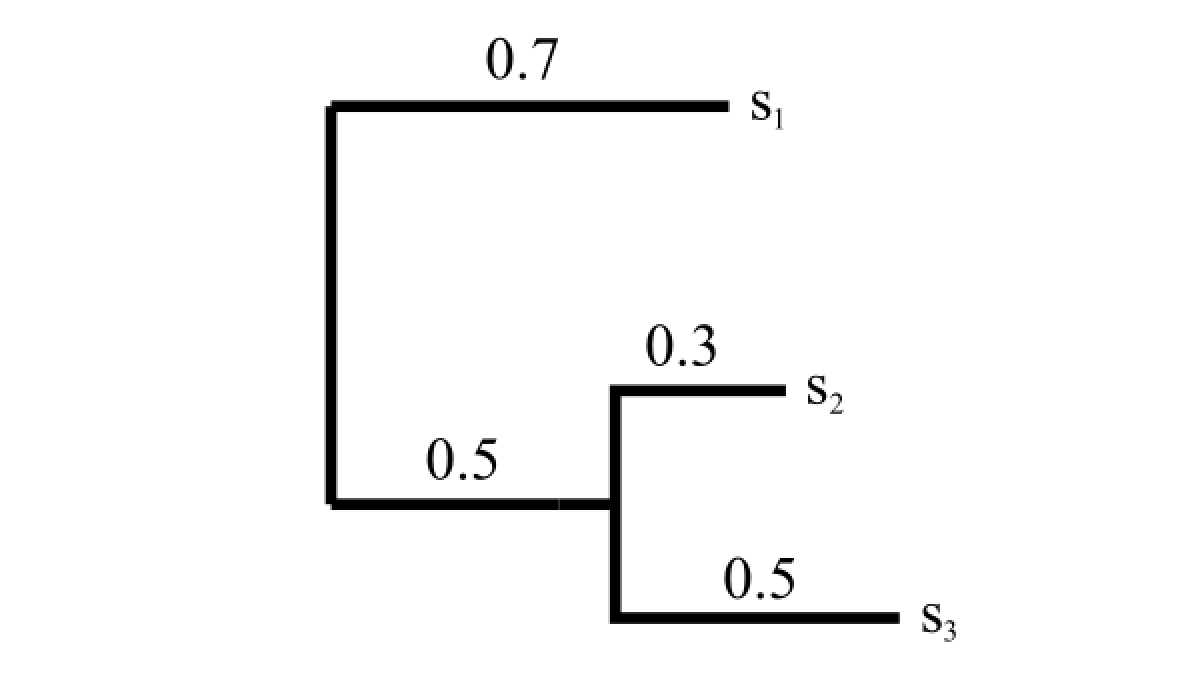
\includegraphics[scale=0.4]{Chapter_PrivatePhylogeneticTrees/tree.png}
        \caption{Example of rooted phylogenetic tree.}
        \label{fig:tree}
    \end{figure}
    
    Therefore, if we consider the equivalence relation, $\sim$, given by
    \begin{equation*}
    (\text{subtree}_1:l_1,\, \text{subtree}_2:l_2)  \sim (\text{subtree}_2:l_2,\, \text{subtree}_1:l_1),
    \end{equation*}
	we have that the quotient set of the trees by $\sim$ satisfy the uniqueness property from an evolutionary point of view.

   
\end{itemize}

For simplicity, denote by $A_d^a$ the private protocol that implements sequentially both functionalities described above, i.e. $A_d^a(s_1, ... , s_m) = \mathtt{A}( \mathtt{DM}(d; s_1, ..., s_m), a)$. This leads to twelve possible combinations of algorithms $A_d^a$ for $d\in\{\text{JC}, \text{K2P}, \text{F84}, \text{LD}\}$ and $a \in \{\text{UPGMA}, \text{NJ}, \text{FM}\}$.

\subsection{Private protocol}

During the distance matrix computation phase ($\mathtt{DM}$) of the private $A_d^a$, each party has to compute the distance between his sequences and the other parties' sequences privately, i.e. without revealing his sequences to the other participating parties. Since this corresponds to several instances of a two-party secure computation, we make use of the Yao protocol described in section~\ref{yaoProtocol}. This means that each party has to generate the boolean circuit representation of the elected distance $d$, which is accomplished by the CBMC-GC software tool before the beginning of the protocol. In section \ref{privDistances}, we analyse how to generate these circuits.

Now, since the Yao protocol is executed only between two different parties $P^i$ and $P^j$ for $i, j \in[n]$, the other participating parties $P^t$, $t\in[n]\setminus \{i,j\}$, do not have access to the distances computed between theses two parties. For this reason, $P^t$ has to receive the result of the Yao protocol execution from both $P^j$ and $P^i$. After this, each party outputs the distance matrix that is used as the input of PHYLIP programs: \texttt{fitch}, \texttt{kitsch} or \texttt{neighbor}. 

In the second phase of the protocol ($\mathtt{A}$), the parties do not need to communicate because this phase only depends on the quantities computed during the first phase. For this reason, this phase is executed internally by each party, who then compute the phylogenetic tree. This phase is carried out by the PHYLIP programs mentioned in the previous paragraph.

These two phases are shown in Figure~\ref{fig:network} and we give more details about the protocol assisted with quantum technologies in the next section. 

\begin{figure}[t]
    \centering
    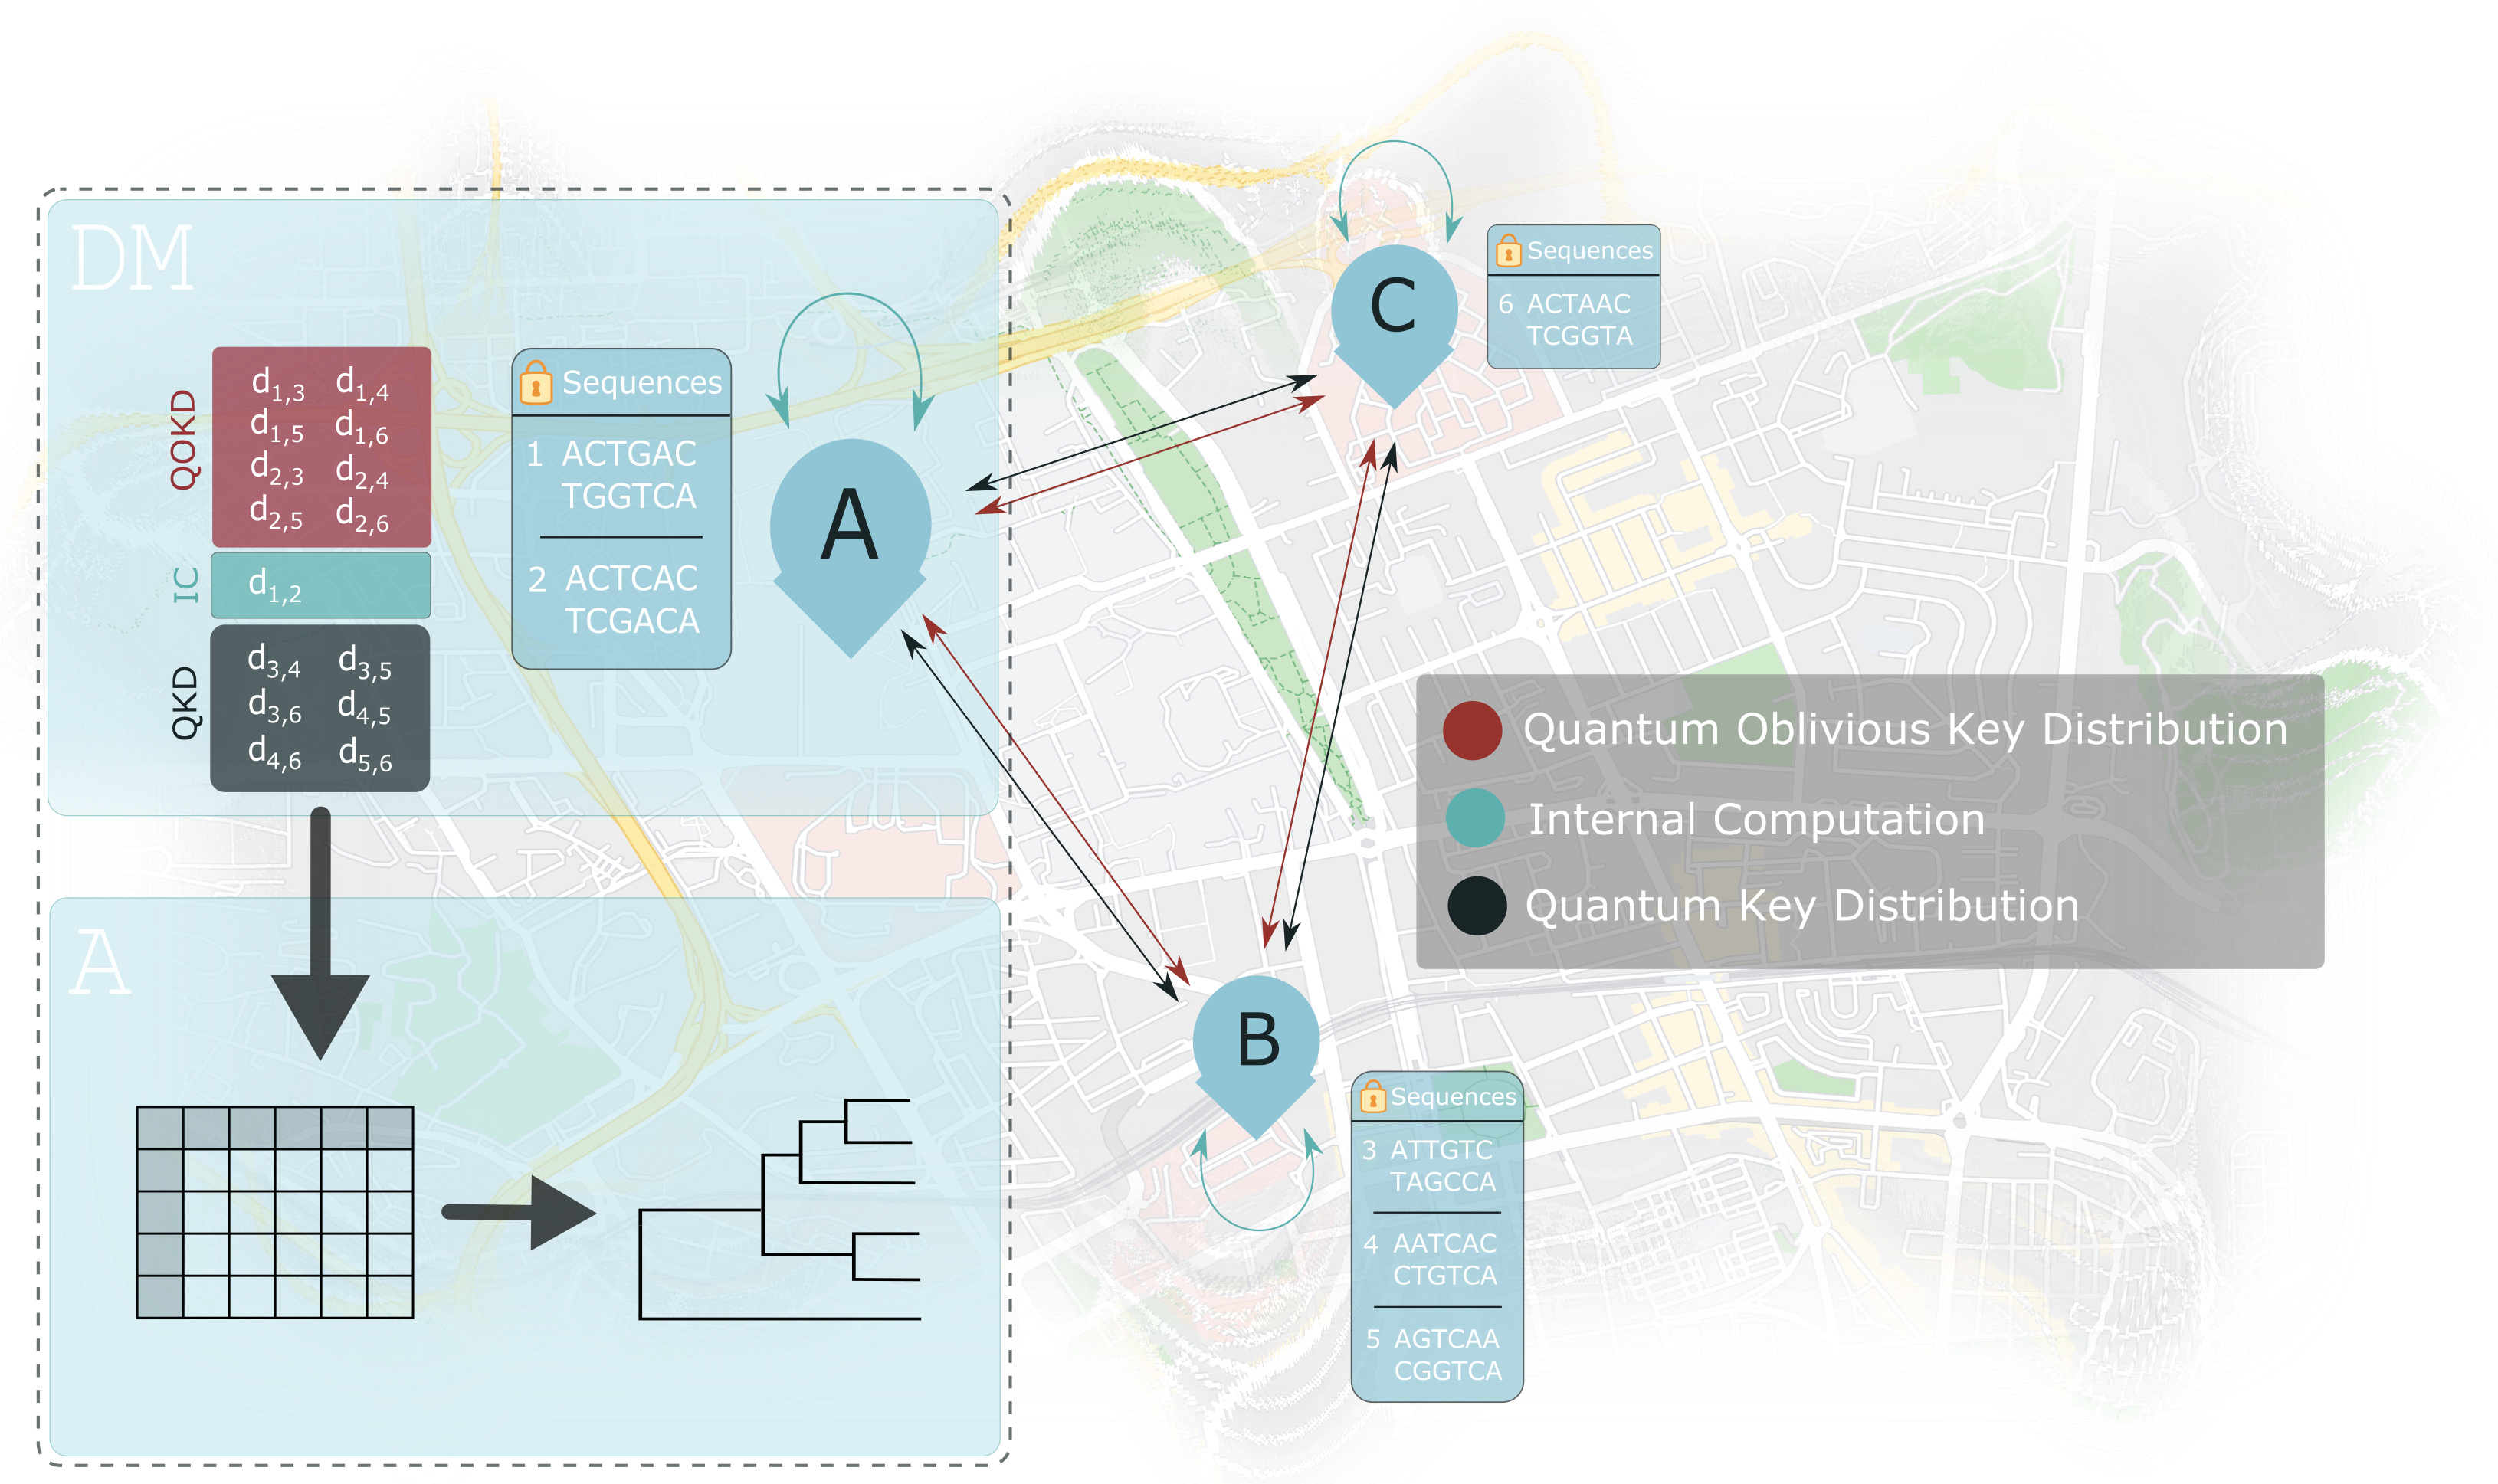
\includegraphics[scale=0.75]{Chapter_PrivatePhylogeneticTrees/PPT.png}
    \caption{Overview of the $A^a_d$ network structure.}
    \label{fig:network}
\end{figure}

\subsection{Quantum private protocol}\label{privProtocol}

Let us specify the private $A_d^a$ protocol with the quantum cryptographic tools. Following the scenario depicted in Figure~\ref{fig:network}, we define $S_i = \{s_{i,1}, ..., s_{i,l}\}$ to be the set of sequences owned by party $P^i$. Also, we denote by $d_{(i,l), (j, k)}$ the distance between the $l$-th sequence of party $P^i$ and the $k$-th sequence of party $P^j$, i.e. $d_{(i,l), (j, k)} = d(s_{i,l}, s_{j,k})$.

As briefly described before, the private $A_d^a$ protocol has two phases. The first phase requires different types of interactions between the parties to compute the desired distance matrix and the second phase is computed internally. Since the second phase is carried out internally, there is no need for communication between the parties. Therefore, the quantum cryptographic tools will only be used during the first private phase. In summary, each pair of parties require two quantum channels as depicted in Figure~\ref{fig:network}: one to generate oblivious keys for oblivious transfer and the other to generate symmetric keys for encryption.

Consider the case where $P_t$ has to compute the distance matrix entry corresponding to distance $d_{(i,l), (j, k)}$. Depending on whether $P_t$ owns both sequences, one of the sequences or none of the sequences $(s_{(i,l)}, s_{(j,k)})$, $P_t$ proceed as follows:

\begin{enumerate}
    \item If $i=j=t$ (i.e. both sequences are owned by $P_t$), $d_{(i,l),(j,k)}$ is computed internally by $P_t$ (blue arrow in Figure~\ref{fig:network});
    \item If $i=t$ and $j\neq t$ (i.e. one of the sequences is owned by $P_t$), $d_{(i,l),(j,k)}$ is computed privately with Yao protocol assisted with QOKD system (red arrow in Figure \ref{fig:network});
    \item If $i\neq t$ and $j\neq t$ (i.e. none of the sequences is owned by $P_t$), both parties $P_i$ and $P_j$ (or just party $P_i$ in case $i=j$) must send to $P_t$ the distance $d_{(i,j),(k,l)}$ encrypted with the symmetric key generated through the QKD system (black arrow in Figure \ref{fig:network}).
\end{enumerate}


\section{Quantum technologies integration}\label{quantumTechIntegration}

Now, let us see the role of quantum technologies in this private system and its integration with quantum networks.

\subsection{Quantum oblivious transfer} \label{quantumTechIntegQOT}

Libscapi implementation of Yao protocol combines a very efficient base OT protocol with one of the fastest OT extension protocols. It uses the base OT (SimpleOT) proposed by Chou and Orlandi \cite{CO15} integrated with the OT Extension (KOS15 \cite{KOS15}) presented in chapter~\ref{classical-and-quantum-OT}. In this setting, the $\Pi^{\textbf{BBCS}}_{\textbf{O}}$ protocol can be implemented in two different ways depending on the number of oblivious keys generated between the two parties: as a base OT protocol integrated within OT extension protocol or as a stand-alone method substituting all Libscapi OT implementation. If the number of oblivious keys generated is scarce compared to the number of OT required, then one should integrate  $\Pi^{\textbf{BBCS}}_{\textbf{O}}$ in the OT extension. Otherwise, one could directly use the  $\Pi^{\textbf{BBCS}}_{\textbf{O}}$ protocol. A scheme of the integration of the quantum oblivious key distribution (QOKD) system is depicted in Figure~\ref{fig:QOKD}.

\begin{figure}[h]
    \centering
    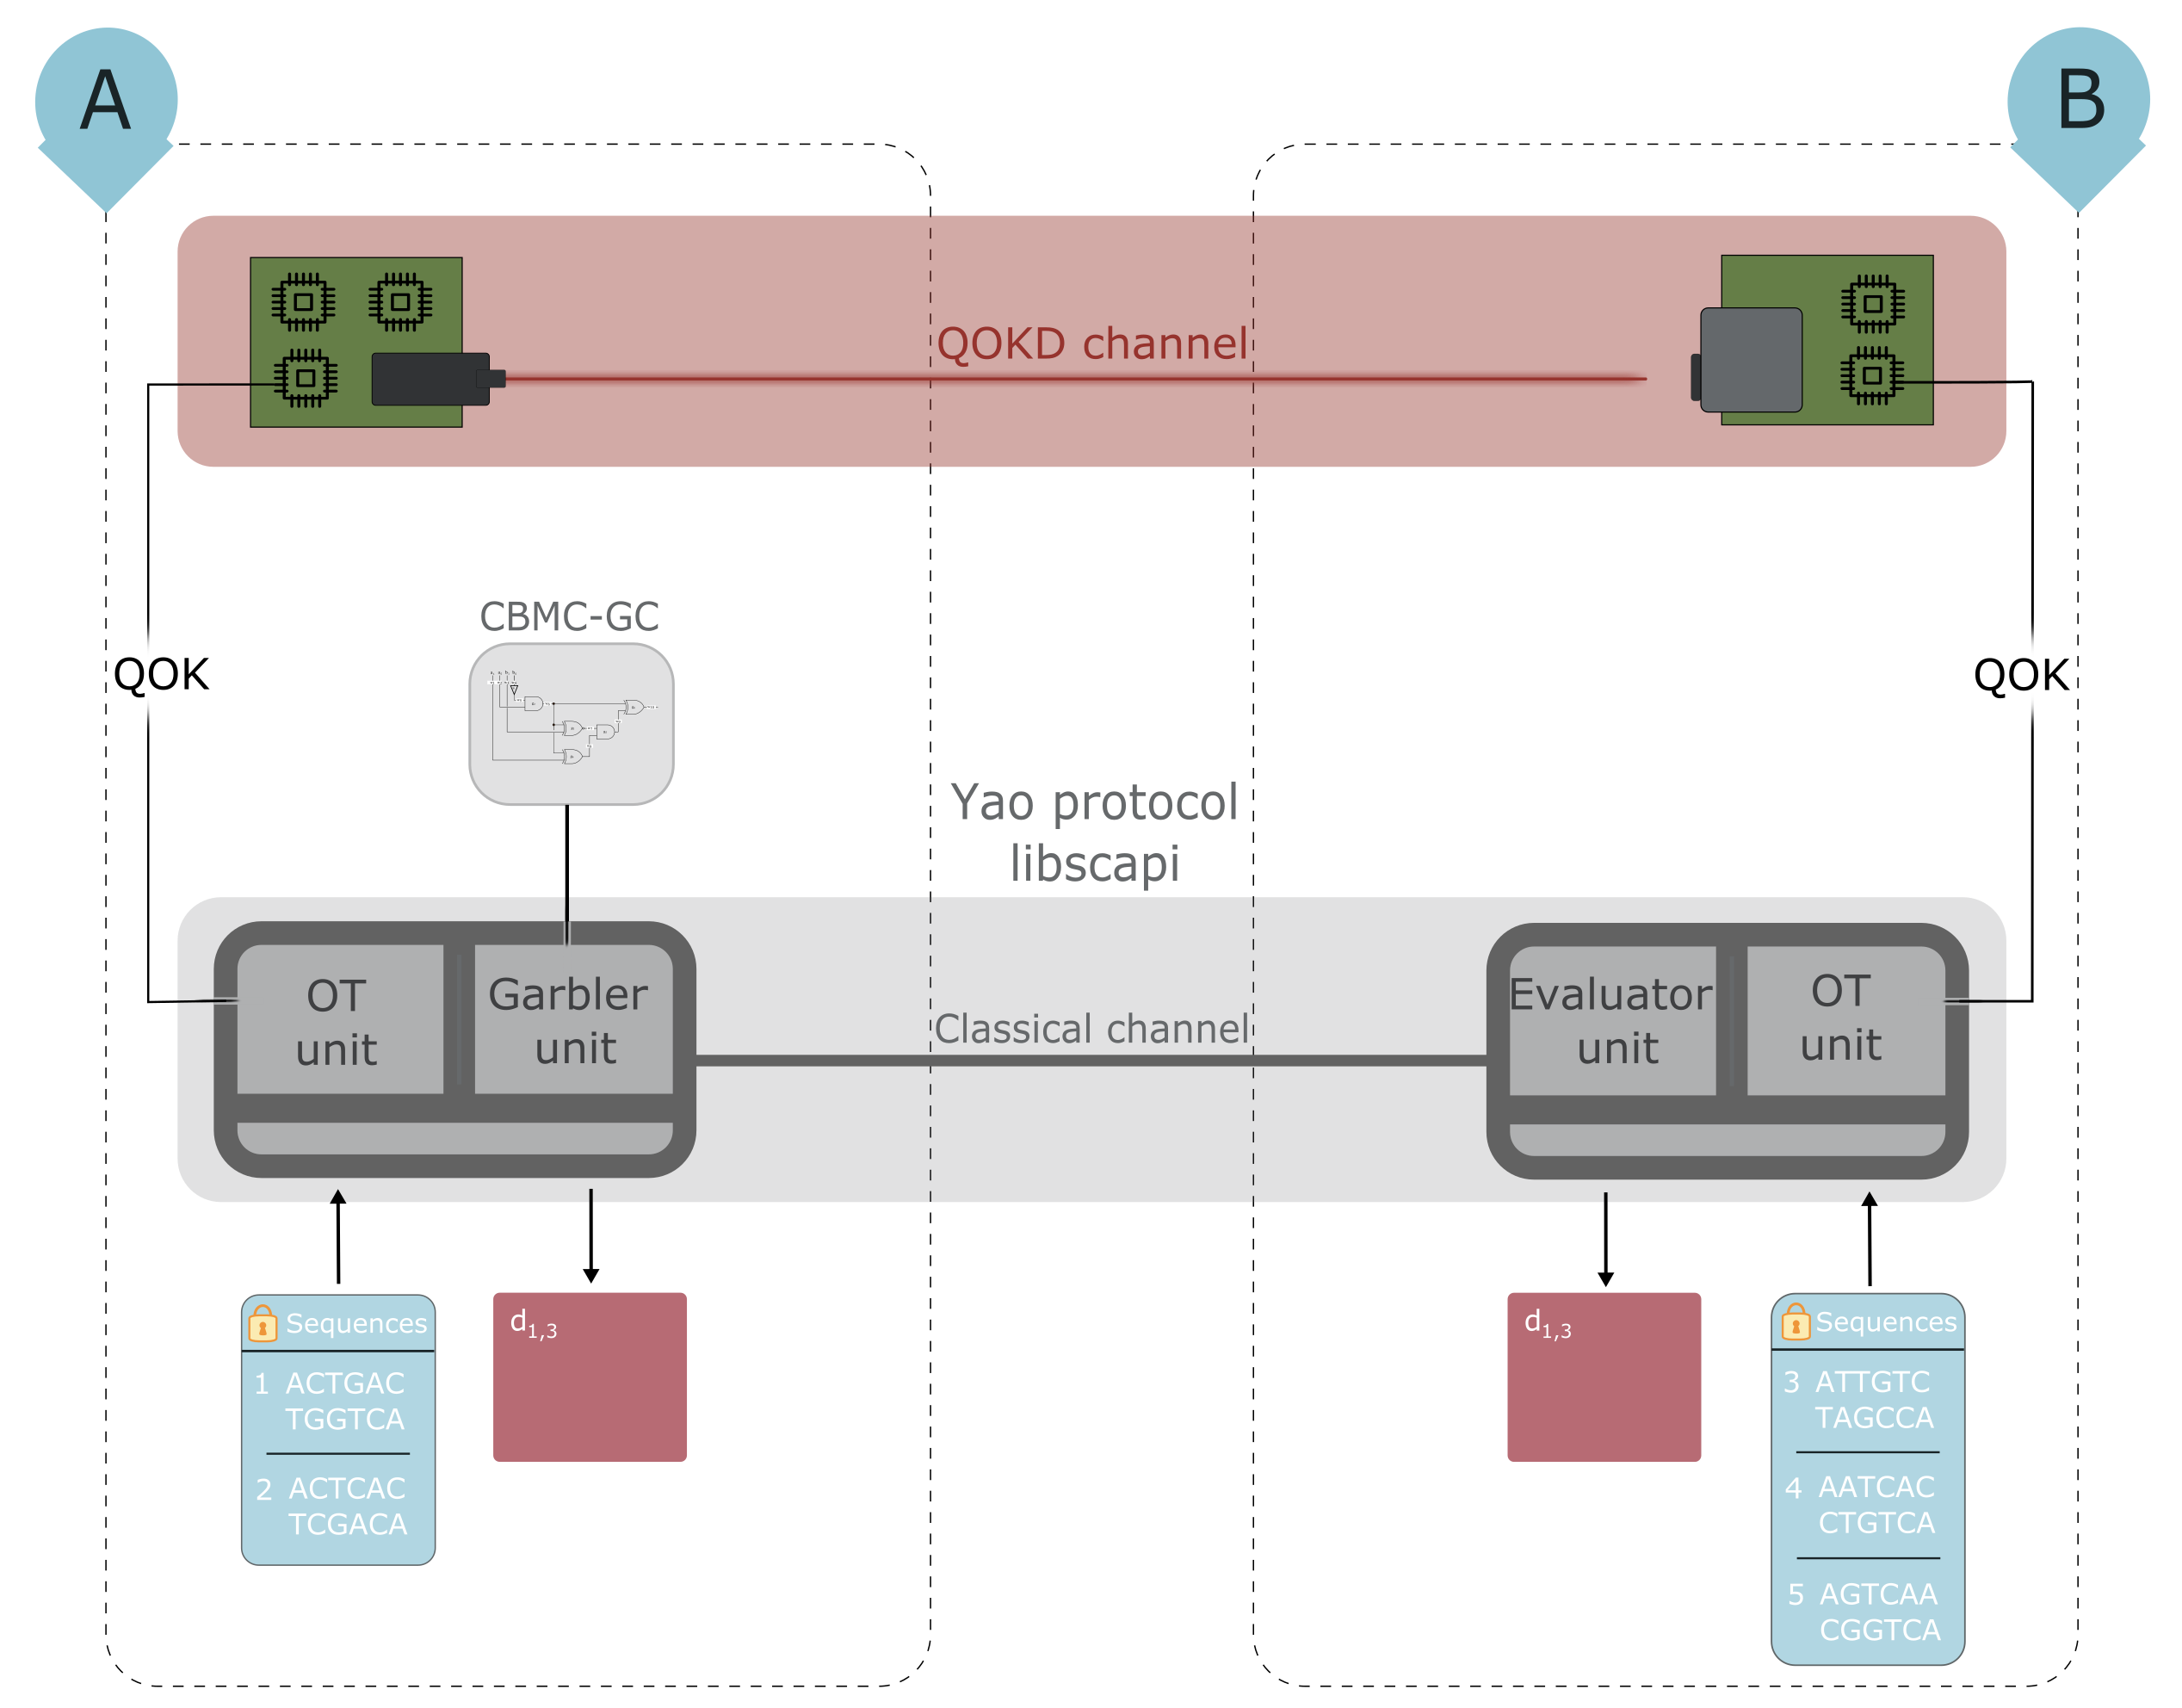
\includegraphics[scale=0.9]{Chapter_PrivatePhylogeneticTrees/QOKD.png}
    \caption{Overview of the integration of the QOKD service and the CBMC-GC tool in the Yao protocol.}
    \label{fig:QOKD}
\end{figure}

It is important to note that the base OTs executed during the pre-computation phase of the OT extension have the parties' roles reversed. This means that the OT extension sender is the base OT receiver and vice-versa. This should be taken into consideration in case the $\Pi^{\textbf{BBCS}}_{\textbf{O}}$ is integrated within OT extension because $\Pi^{\textbf{BBCS}}_{\textbf{O}}$ is not symmetric in the sense that the apparatus used by the sender is different from that of the receiver. However, since it is known that OT is symmetric, we can use the reduction proposed in \cite{Wolf2006} without having to swap the quantum technological material.

\subsection{Quantum random number generation} 

As previously described, the Yao protocol needs to generate random numbers for the keys in the \textit{Wire encryption} step. This is crucial for the security of the protocol because its predictability allows deducing the parties' input as reported in \cite{ALSZ13}. 

Libscapi implementation makes use of OpenSSL library function \texttt{RAND\_bytes} to randomly generate a seed from which it computes new numbers. In this private system, we substitute this function to a call of QRNG.

\subsection{Quantum key distribution} 

The QKD system allows the participating parties to receive the distance elements of the sequences they do not own, while preserving the security of the system. We use the keys generated by the QKD system along with the perfect cipher: one-time pad. %with the OpenSSL AES-CTR implementation present in Libscapi library. 


\subsection{Quantum network integration}

\subsubsection{Technological equipment}

Both QKD and QOKD protocols rely on the same physical processes. They can both be realized either with continuous or discrete variables \cite{Pirandola2020,Silva2019,FGSPSW18, Lemus20}. Also, the technological equipment used by the receiver (Bob) and transmitter (Alice) is the same in both quantum services (QKD and QOKD). As for the case of the prepare-and-measure setting, the first quantum step is the same in both protocols: Alice randomly sends quantum states in two different bases and Bob measures these states on random bases. The difference relies on the classical post-processing phase. So, we can conclude that both services share the same technological equipment (fibre, receiver and transmitter). Moreover, as proposed by Pinto et al. \cite{Pinto2020} in a similar setting, both QKD and QOKD services can coexist with classical signals in the same fibre.

\subsubsection{Network topology}

The quantum private protocol explained above in section~\ref{privProtocol} assumes that every two parties have a direct quantum channel between them that is used to generate oblivious keys and symmetric keys, i.e. a fully connected quantum network. This approach follows from the fact that the first QKD and quantum OT (QOT) protocols were based on prepare-and-measure techniques \cite{BB84, BBCS92}. However, as discussed in chapter~\ref{chapter_QOT}, there are also protocols that implement device-independent QOT (DI-QOT) \cite{KW16, RW20} (under some constraints) and DI-QKD \cite{Pirandola2020}. In addition to the advantages from a security point of view, these DI protocols can also be implemented within a star-structured quantum network having an untrusted party as the middle point. This increases the implementation flexibility of the proposed quantum private protocol of phylogenetic trees (section~\ref{privProtocol}).

As analysed by Joshi et al. \cite{JAW20}, existing networks fall into three possible types: trusted node networks, actively switched and fully connected quantum networks based on entanglement sharing and wavelength multiplexing. Using the two types of protocols just mentioned (prepare-and-measure and device-independent), it is possible to implement our proposed system in all three existing quantum network implementation types.

Moreover, Kumaresann et al. \cite{KRS16} analyses possible SMC infrastructure topologies that can be created based on a set of OT channels shared between some pairs of parties in the network. They developed ``secure protocols that allow additional pairs of parties to establish secure OT correlations using the help of other parties in the network in the presence of a dishonest majority" (Abstract, \cite{KRS16}). Since they work in the information-theoretical setting, there is no security loss in combining Kumaresann protocol with quantum approaches. This integration increases the range of configurations allowed. However, further efficiency analysis has to be done to understand the impact of this approach in practice.



\section{System security}\label{systemSecurity}

In this section, we analyse the security of the proposed system. We start by describing the methods used to privately compute the distance between two sequences and then we prove the security of the private protocol proposed in section~\ref{privProtocol} which implements the functionality described in section~\ref{Functionality}.


\subsection{Private computation of distances} \label{privDistances}

The private computation of the distance between sequences is an important building block in the security of the system. We have that the privacy of the sequences directly relies on this step. Here, we go through the methods used to compute the distances used by the PHYLIP program: Jukes-Cantor, Kimura 2-parameter, F84 and LogDet.

A common building block to all these four distance metrics is the computation of the Hamming distance between two sequences $x$ and $y$, $h_{xy}$. We start by looking at an adapted divide-and-conquer way to compute the Hamming distance between two sequences and then we see how to apply it to the private computation of distance metrics.

\subsubsection{Hamming distance}

We are interested in the boolean representation of the Hamming distance and, as mentioned above, we use the CBMC-GC tool to translate ANSI-C code into this representation. Usually, to compute the Hamming distance between two binary strings, $x$ and $y$, we start by applying the XOR operation, $z = x \oplus y$. Then, we just have to count the number of $1$'s in $z$. This operation is commonly known as population count or $\text{popcount}(z)$ for short. So, the binary Hamming distance is given by $h_{xy} = \text{popcount}(x \oplus y)$.

We use an adapted divide-and-conquer technique for the computation of $\text{popcount}(z)$ \cite{W12}. Originally, this divide-and-conquer technique starts by dividing the sequence into 2-bit blocks and then counts the number of $1$'s inside each 2-bit block. After that, it allocates the result of each block in a new 2-bit block. Then, we can sum the values inside these 2-bit blocks iteratively. %\ref{https://arxiv.org/pdf/1611.07612.pdf}. 

We follow the approach described above but we have to tailor it for the computation of the Hamming distance between two four-based sequences $(A, C, G, T)$. Since we are using a boolean circuit representation, the nucleotide sequences must be represented in binary. So, by convention, we use the following 2-bit encoding: $A = 00$, $C=01$, $G=10$ and $T=11$. If we follow directly the approach described above, we would have that the Hamming distance between the single-valued sequences $``A"$ and $``C"$ is smaller than the single-valued sequence between $``A"$ and $``T"$:
\begin{eqnarray*}
h(A, C) &=& \text{popcount}(00 \oplus 01)\\
&=& \text{popcount}(01) = 1,
\end{eqnarray*}
\begin{eqnarray*}
h(A, T) &=& \text{popcount}(00 \oplus 11)\\
&=& \text{popcount}(11) = 2.
\end{eqnarray*}

This issue comes from the fact that we are counting the number of $1$'s inside every 2-bit blocks. Instead, we are just interested in knowing if there is at least one element 1 inside each 2-bit block because it indicates that the bases at that site are different. Therefore, before counting the number of 1's in the \texttt{XOR}ed sequence, we apply an \texttt{OR} operation to the bits inside every 2-bit blocks. We call this operation $\text{popcount}^t(z)$. For simplicity, hereafter we denote by $h_{xy}$ the tailored Hamming distance between sequences $x$ and $y$. Now, we have that the tailored Hamming distance between $``A"$ and $``T"$ gives the desired result:
\begin{eqnarray*}
h(A, T) &=& \text{popcount}^t(00 \oplus 11)\\
&=& \text{popcount}^t(11) \\
&=& \text{popcount}\big(\texttt{OR}(1,1)\big) = 1.
\end{eqnarray*} In Figure~\ref{fig:hamming_divide}, we show an example on how to compute the Hamming distance between two-valued sequences $``AG"$ and $``GC"$.

\begin{figure}[h]
    \centering
    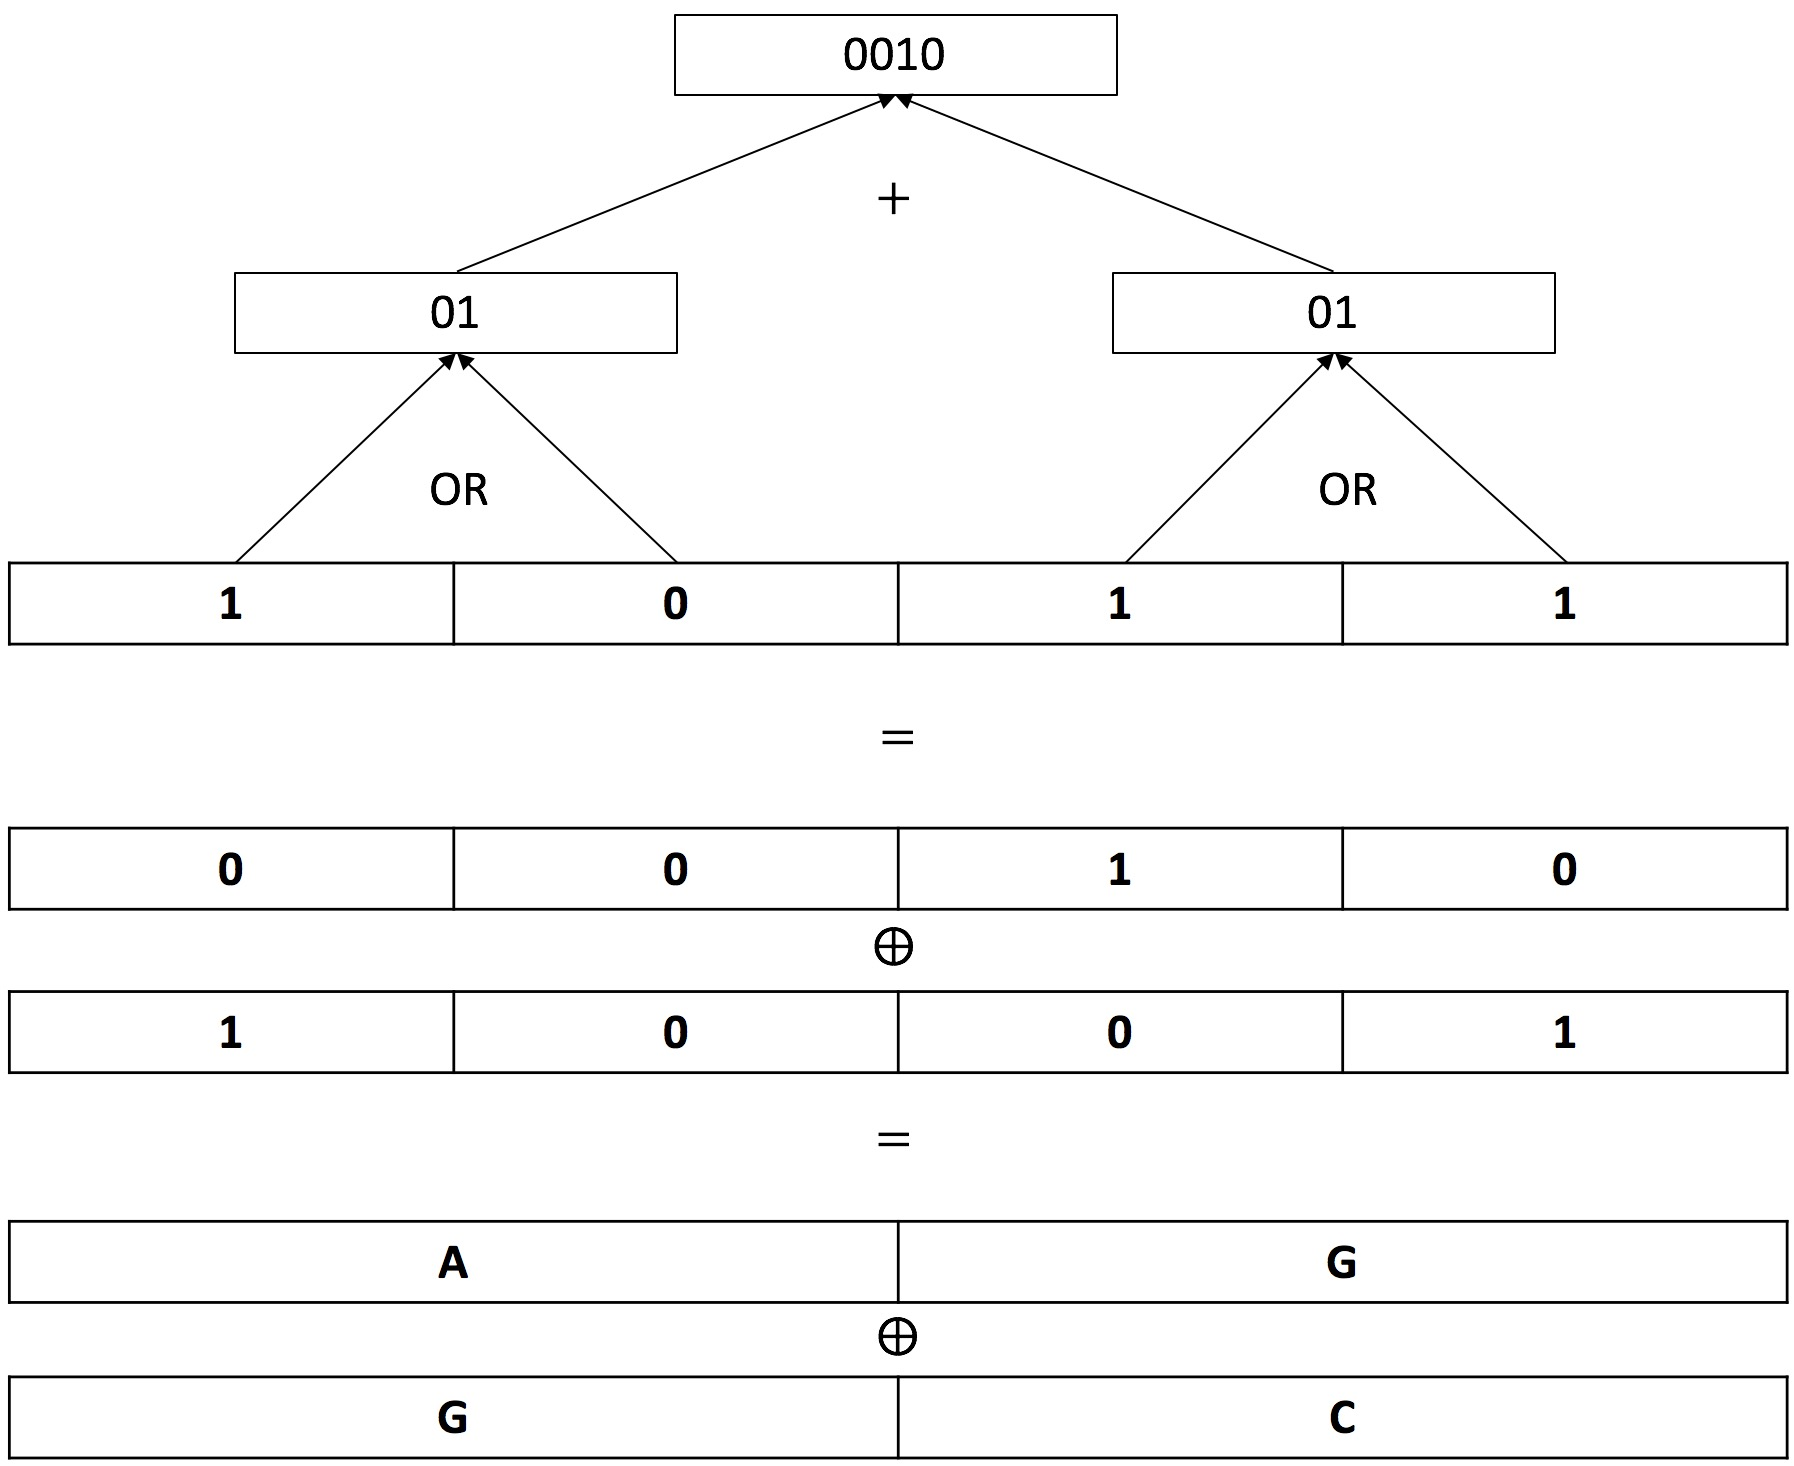
\includegraphics[scale=0.12]{Chapter_PrivatePhylogeneticTrees/divide-and-conquer-tailored.jpeg}
    \caption{Overview of the tailored divide-and-conquer technique. This corresponds to lines \texttt{12-19} in Figure~\ref{fig:jc_cbmc-gc} in Appendix~\ref{appendix:appendixA}.}
    \label{fig:hamming_divide}
\end{figure}


\subsubsection{Jukes-Cantor} 
As described in section \ref{JK_model}, the Jukes-Cantor distance between two sequences is given by:
$$d_{xy} = -\frac{3}{4} \ln \Big(1- \frac{4}{3}\frac{h_{xy}}{N}\Big),$$
where $h_{xy}$ is the hamming distance between sequence $x$ and sequence $y$.

Now, note that the function $f(x) = -\frac{3}{4} \ln \Big(1- \frac{4}{3}\frac{x}{N}\Big)$ is one-to-one. This means that, from a privacy point of view, $f(x)$ carries the same amount of information than $x$. Therefore, we could simply proceed as follows:

\begin{enumerate}
    \item Privately compute the Hamming distance, $h_{xy}$, using the tailored Hamming distance method described above and the Yao protocol assisted with quantum oblivious keys;
    \item Internally compute $d_{xy} = f(h_{xy})$ (no need of quantum SMC).
\end{enumerate}

This way, we just have to generate the boolean circuit for $h_{xy}$ rather than generating for the full expression $d_{xy}$.


\subsubsection{Kimura}
In section~\ref{K2P_model}, we saw that the Kimura 2-parameter model leads to the following distance:
$$d_{xy} = -\frac{1}{2}\ln\bigg( \big(1-2P-Q\big) \sqrt{1-2Q} \bigg),$$
where $P=\frac{n_1}{N}$, $Q=\frac{n_2}{N}$ and $n_1$ and $n_2$ are respectively the number of sites for which two sequences differ from each other with respect to type I ("transition" type) and type II ("transversion" type) substitutions.

Similar to the case of Jukes-Cantor metric, note that $h(x) = -\frac{1}{2}\ln(\sqrt{\frac{x}{N^3}})$ is one-to-one and only defined for $x>0$. Thus, we can proceed as follows:

\begin{enumerate}
    \item Privately compute the expression $c = (N-2n_1-n_2)^2(N-2n_2)$ using the tailored Hamming distance method described above and the Yao protocol assisted with quantum oblivious keys;
    
    \item Internally computes $d_{xy} = h(c)$ (no need of quantum SMC).
\end{enumerate}

More precisely, the ANSI-C code that privately computes expression $c = (N-2n_1-n_2)^2(N-2n_2)$ proceeds as follows. It uses the function $\text{popcount}_t(z)$ described above to compute the quantities $n_1$ and $n_2$. Observe that a transition type ($A\leftrightarrow G$ or $C\leftrightarrow T$) renders the same XOR value:
\begin{eqnarray*}
A \oplus G = 00 \oplus 10 = 10  \\
T \oplus C = 11 \oplus 01 = 10 .  
\end{eqnarray*}

Therefore, using a four-sized sequence, the quantities $n_1$ and $n_2$ are given by:
\begin{eqnarray*}
n_1 &=& 4 - \text{popcount}_t(x\oplus y\oplus 10101010)\\
n_2 &=& \text{popcount}_t(x\oplus y) - n_1.
\end{eqnarray*}

%Again, we use the Yao protocol assisted with QOK for an expression with basic operations.

%Etc. Also comment on the limits. Ex: $32000^3$ needs 45 binary digits to be represented. Therefore the output should be a long int (64 bit) and not just int. Otherwise there will be overflow. 



\subsubsection{F84 and LogDet}
Recall from section \ref{evolDist}, that the F84 ($F_{xy} $) and LogDet ($L_{xy} $) distances are given, respectively, by:
\begin{equation}
    F_{xy} = -2 A\ln\bigg( 1- \frac{P}{2A} - \frac{(A-B)Q}{2AC} \bigg) + 2(A-B-C)\ln\bigg( 1-\frac{Q}{2C} \bigg),
\label{eq:F84_distance}
\end{equation}
\begin{equation}
    L_{xy} = -\frac{1}{4}\ln\Bigg( \frac{\det F_{xy}}{\sqrt{\det \prod_x \prod_y}} \Bigg),
\label{eq:LogDet_distance}
\end{equation}
where $A = \frac{\pi_C \pi_T}{\pi_Y} + \frac{\pi_A \pi_G}{\pi_R}$, $B=\pi_C\pi_T + \pi_A\pi_G$ and $C=\pi_R\pi_Y$ for $\pi_Y = \pi_C + \pi_T$ and $\pi_R = \pi_A + \pi_G$, and $P$ and $Q$ are defined as in the Kimura 2-parameter mode above. Also, the divergence matrix $F_{xy}$ is a $4\times 4$ matrix such that the $ij-$th entry gives the proportion of sites in sequence $x$ and $y$ with nucleotide $i$ and $j$, respectively. Also, $\prod_x$ and $\prod_y$ are diagonal matrices where its $i-$th component correspond to the proportion of $i$ nucleotide in the sequence $x$ and $y$, respectively.

As before, we want to split the private computation of both $F_{xy}$ and $L_{xy}$ in two steps. Note that, in this case, there is no clear way to define two bijective functions, $g()$ and $q()$, on some simple parameters, $d$ and $e$, such that $F_{xy} = g(d)$ and $L_{xy} = p(e)$. By simple parameters, we mean parameters that do not depend on complex operations such as logarithm or square root. Instead, one can use the CORDIC algorithm \cite{V59, Songhori2019} for square-roots and logarithm functions and translate an approximation of both $F_{xy}$ and $L_{xy}$ into boolean circuits.



\subsection{Private computation of phylogenetic trees}

In this section, we prove that the protocol $A^a_d$ described in section~\ref{privProtocol} securely implements functionality $\mathtt{A}\circ \mathtt{DM}$ described in section~\ref{Functionality} according to the security definition~\ref{def:security}. So, we want to prove the following theorem:

\begin{theorem}
The protocol $A^a_d$ securely realizes $\mathtt{A}\circ \mathtt{DM}$ in the presence of semi-honest adversaries.
\end{theorem}

We start by noting that the ideal functionality outputs the distance matrix to the parties and that during $\mathtt{A}$ computation there is no interaction between the parties. Therefore, the security of the system is independent of the distance-based algorithm used (UPGMA, Neighbour-Joining or Fitch-Margoliash) and we can only focus on the computation of $\mathtt{DM}$ functionality.

As already mentioned, the protocol that implements the functionality $\mathtt{DM}$ is built up by many invocations of a two-party distance functionality, denoted by $\mathtt{D}_d$ for $d\in\{\text{JC}, \text{K2P}, \text{F84}, \text{LD}\}$. So, in order to prove the above theorem, we will need to following two lemmas:

\begin{lemma}\label{firstlemma}
$A^a_d$ privately reduces $\mathtt{DM}$ to $\mathtt{D}_d$, i.e. an oracle-aided $A^a_d$ protocol privately computes $\mathtt{DM}$ using the oracle-functionality $\mathtt{D}_d$.
\end{lemma}

\begin{proof}
In order to prove this lemma, we have to develop a simulator $Sim$ that simulates the view of a set of corrupted parties $C$. The $Sim$ starts from receiving all the input sequences from the corrupted parties. It then proceeds as follows:

\begin{enumerate}
    \item Generates random sequences of the honest parties, $H$.
    \item Invokes the oracle-functionality $\mathtt{D}_d$ on these sequences.
    \item Sends to all corrupted parties $C$ the results of distances computed from honest parties sequences
    \item Invokes the oracle-functionality $\mathtt{D}_d$ on the sequences owned by the corrupted parties.
    \item Invokes the oracle-functionality $\mathtt{D}_d(s_i, s_j)$ for $s_i\in H$ and $s_j\in C$. 
\end{enumerate}

In a real execution, the corrupted parties will only receive the distances computed by $\mathtt{D}_d$ on the honest parties sequences (as in step 2.), on their sequences (as in step 4.) and between corrupt and honest parties. Therefore, we have that the oracle-aided $A^a_d$ protocol privately computes $\mathtt{DM}$ using the oracle-functionality $\mathtt{D}_d$.

\end{proof}

\begin{lemma}\label{secondlemma}
Yao protocol with the OT primitive instantiated by $\Pi^{\textbf{BBCS}}_{\textbf{O}}$ protocol (Figure~\ref{fig:BBCS_Transfer}) privately computes $\mathtt{D}_d$.
\end{lemma}

\begin{proof}

In \cite{FS09} it was developed a framework that allows quantum protocols to be composed in a classical environment. They also mention that a general secure function evaluation remains secure when instantiating the OT primitive by a secure quantum version. In \cite{DFL+09}, it was proved that $\Pi^{\textbf{BBCS}}_{\textbf{O}}$ protocol is secure according to the security definition given in \cite{FS09}. Therefore, we can compose the $\Pi^{\textbf{BBCS}}_{\textbf{O}}$ protocol with a Yao protocol \cite{Lindell2008} while preserving the overall security. 

\end{proof}

So, from Lemma \ref{firstlemma} and \ref{secondlemma} we can use the composition theorem \ref{compositionthm} and conclude that the protocol $A^a_d$ is secure.

We have proved that our system is well designed and secure against quantum computer attacks under the semi-honest model. In order to extend the protocol to the malicious setting, we just have to implement a two-party secure computation protocol that is secure in the malicious adversary model \cite{Evans2018}. 




\section{Complexity analysis}\label{CompleAnalysis}

%\hl{ explicar melhor aqui que vamos primeiro fazer uma comparação da análise de complexidade entre os dois casos e depois vamos avaliar experimentalmente na secção seguinte.}

In this section, we start by analysing the complexity of the protocol $A^a_d$ presented before. We assume there are $n$ parties, $P^1, \ldots, P^n$, with $M_1, \ldots, M_n$ sequences, respectively. Also, we assume that the sequences are aligned and that they have the same number of nucleotides, $s$.

% In this section we start by comparing the computation and communication complexity of the fastest reported malicious oblivious extension protocol implemented in Libscapi library \cite{K15} and the optimized version of $\Pi^{\textbf{BBCS}}_{\textbf{O}}$ presented in \cite{SPM21}. Then, we analyse the complexity of the protocol $A^a_d$ presented before. We assume there are $n$ parties, $P^1, ..., P^n$, with $M_1, ..., M_n$ sequences, respectively. Also, we assume that the sequences are aligned and that they have the same number of nucleotide, $s$. 

\subsection{Protocol complexity analysis}\label{compAnalysis}

Now, let us analyse the complexity of the protocol presented in section \ref{privProtocol}. 

\subsubsection{Yao protocol executions}
Regarding the number of Yao protocol executions, we have that each party $P^j$ owning $M_j$ sequences has to perform $N_{\text{Yao}}^j = M_j\sum_{i\neq j} M_i$ secure distance computations. So, the total number of Yao protocol executions is given by
$$N_{\text{Yao}} = \sum_j N_{\text{Yao}}^j = \sum_{j, i\neq j} M_j M_i.$$
If we assume the number of sequences per party to be the same, i.e. $M_j = M\, \forall j\in[n]$, then we can simplify the expression above and conclude that $N_{\text{Yao}} = M^2 n(n-1)$. This means that the number of Yao protocol executions is quadratic in the number of sequences per party ($\mathcal{O}(n^2)$) and also in the number of parties ($\mathcal{O}(M^2)$). 

\subsubsection{OT executions}
From $N_{\text{Yao}}$ we can deduce the number of OT executions. In the Yao protocol, we need to execute one OT for each of the evaluator's input wires. For a sequence with $s$ nucleotides and using a two-bit representation of each nucleotide, the boolean circuit that computes the distance between two sequences will have $2s$ input wires for each party input. Therefore, each party executes the following number of OT executions ($\forall j$):
\begin{eqnarray*}
N_{\text{OT}}^j &=& N^j_\text{Yao} \cdot 2s \\
&=& 2sM^2(n-1).
\end{eqnarray*}

It is important to note that $N_{\text{OT}}^j$ is independent of the size of the boolean circuit used, i.e. it is independent of the distance metric $d$ used in the protocol. This is a consequence of using the Yao protocol where the number of OT only depends on the input size. In case we were using GMW \cite{Goldreich87} protocol, the number of OT per party would depend on the size of the circuit.

As mentioned in section \ref{quantumTechIntegQOT}, in case the number of oblivious keys generated is scarce compared to the number of OT required, we can use the $\Pi^{\textbf{BBCS}}_{\textbf{O}}$ protocol to generate the base OT used within OT extension protocol. In this case, we just have to generate $\kappa$ $\Pi^{\textbf{BBCS}}_{\textbf{O}}$ protocols per Yao execution: $L^j_\text{bOT} = N^j_\text{Yao} \cdot \kappa = \kappa M^2(n-1)$.

\subsubsection{Oblivious keys}
At this point, we can easily deduce the size of oblivious keys that each pair of parties have to generate when using messages of size $l$. 

In case we use $\Pi^{\textbf{BBCS}}_{\textbf{O}}$ protocol to generate the final OT:
\begin{eqnarray*}
L^j_{\text{ok}} &=& N_{\text{OT}}^j \cdot 2l \\
&=& 4slM^2(n-1).
\end{eqnarray*}

Also, we can use the number of OT executions per party and the analysis from Table~\ref{table:complexity} and \cite{SPM21} to compute the computational and communication complexity (in bits) of $\Pi^{\textbf{BBCS}}_{\textbf{O}}$:
\begin{eqnarray*}
\mathcal{C}^j_{\text{comp}} &=&  N_{\text{OT}}^j \cdot 8l \\
&=& 16 slM^2(n-1),
\end{eqnarray*}
\begin{eqnarray*}
\mathcal{C}^j_{\text{comm}} &=&  N_{\text{OT}}^j \cdot 3l \\
&=& 6 slM^2(n-1).
\end{eqnarray*}

In case we use $\Pi^{\textbf{BBCS}}_{\textbf{O}}$ protocol to generate the base OT, the total size of oblivious key required is:
\begin{eqnarray*}
L^j_{\text{bok}} &=& N_{\text{bOT}}^j \cdot 2l \\
&=& 2\kappa lM^2(n-1).
\end{eqnarray*}


\subsubsection{QRNG}
The QRNG has to generate twice the total length of oblivious keys, i.e. $L_{\text{QRNG}} = 2L_\text{ok}$.

\subsubsection{Internal computation}
Number of internal computations per party:
$$N_\text{int}^j = \binom{M}{2} = \frac{M!}{2!(M-2)!}.$$

\subsubsection{Encryption keys}
As discussed before, for every party $P^j$, $P^t$ ($t\neq j$) has to receive from $P^j$ the distances known by $P^j$ that $P^t$ does not have access. So, $P^j$ has to send $M^2(n-2) + N_\text{int}^j$ distance values to $P^t$. Consequently, the length of the QKD key used to send these distances to $P^t$ is:
$$32(M^2(n-2) + N^j_\text{int}),$$
for a $32-$bit number representation. Therefore, the total size of key shared between two parties $P^j$ and $P^t$ must be:
$$L^{jt}_{qkd} = 64(M^2(n-2) + N_\text{int}).$$

Also, each party must have an overall shared key of $L^{j}_{qkd} = \sum_{i\neq j} L^{i}_{qkd} = 64(n-1)(M^2(n-2) + N^j_\text{int})$.

% Dizer a que é que corresponde este cenário (!!) 


\subsection{Use case}\label{useCase}

We now present the scenario used to test and compare both quantum-assisted and classical-only approaches. We start by exploring the complexity analysis and the OT comparison carried out in previous sections. We extend this analysis in the next section with a testbed implementation. 

We consider a scenario where three parties $n=3$ have $M$ SARS-CoV-2 genome sequences (with length $s=32\,000$) and want to privately compute a phylogenetic tree from them. In the next section we consider a varying number of sequences, but, for now, we set $M=10$. Following a standard choice \cite{ALSZ13}, we consider garbled circuit keys with $l = 128$ bits, computational security parameter with $\kappa = 128$ bits and statistical security parameter with $w = 64$ bits. For these parameter values, we can instantiate the expressions deduced in the complexity analysis (section~\ref{compAnalysis}). This information is summarized in Table~ \ref{table:phylo_tree_complexity}. As expected, the total size of oblivious keys ($L^j_{\text{ok}}$) required for a scenario where $\Pi^{\textbf{BBCS}}_{\textbf{O}}$ is the main OT protocol is three orders of magnitude higher than the case where $\Pi^{\textbf{BBCS}}_{\textbf{O}}$ serves as a base OT protocol in KOS15 ($L^j_{\text{bok}}$). Also, we note that the total size of symmetric keys required in the protocol ($L^j_{qkd}$) is much smaller than that of oblivious keys ($L^j_{\text{ok}}$ and $L^j_{\text{bok}}$), pointing to the fact that its management should be less expensive than the oblivious keys management system. This will be discussed further in the next section.

\begin{table*}[t]
\centering
\begin{tabular}{lccc}
\toprule
Parameter & Formula & Amount & Generation Time \\ 
\midrule
$L^j_{\text{ok}}$ & $4slM^2(n-1)$ & $3.3 \times 10^9$ bit & $5\text{m}30\text{s}$ \\ 
$L^j_{\text{bok}}$ & $2\kappa lM^2(n-1)$ & $6.6 \times 10^6$ bit & $0.64\text{s}$ \\ 
$L^j_{\text{QRNG}}$ & $8slM^2(n-1)$ & $6.6 \times 10^9$ bit & $28$s \\ 
$L^{j}_{qkd}$ & $64(n-1)(M^2(n-2) + \binom{M}{2})$ & $18.6 \times 10^3$ bit & $1.9\times 10^{-3}$s \\
$N^j_{\text{Yao}}$ & $M^2(n-1)$ & $200$ &  \\ 
$N^j_{\text{OT}}$ & $2sM^2(n-1)$ & $12.8 \times 10^6$ &  \\ 
$N^j_{\text{bOT}}$ & $\kappa M^2(n-1)$ & $25.6 \times 10^3$ &  \\
$N^j_{\text{int}}$ & $\binom{M}{2}$ & $45$ &  \\ 
\bottomrule
\end{tabular}
\caption{Complexity analysis where $n=3$, $M=10$, $s=32\,000$ and $l, \kappa=128$. $L^j_{\text{ok}}$: size of total oblivious key. $L^j_{\text{bok}}$:  total size of oblivious key for base OT. $L^j_{\text{QRNG}}$: random bits generated by QRNG. $L^{j}_{qkd}$: total size of QKD keys. $N^j_{\text{Yao}}$: number of Yao protocol executions. $N^j_{\text{OT}}$: number of OT executions. $N^j_{\text{bOT}}$: number of base OT executions. $N^j_{\text{int}}$: number of internal computations.}
\label{table:phylo_tree_complexity}
\end{table*}

We can also estimate the time required to generate the keys based on their size. If we consider state-of-the-art rates of 10 Mbit/s for both QKD and QOKD systems \cite{YPT18} and a rate of 240 Mbit/s for QRNG (ID Quantique QRNG PCIe cards \cite{IDQ}), we would need around $5\text{ minutes}$ for $L^j_{\text{ok}}$, $0.64\text{s}$ for $L^j_{\text{bok}}$, $28$s for $L^j_{\text{QRNG}}$ and $1.9\times 10^{-3}$s for $L^{j}_{qkd}$. Note that we can significantly reduce the time of the precomputation phase in case we integrate $\Pi^{\textbf{BBCS}}_{\textbf{O}}$ with KOS15 OT extension protocol. 

%Finally, we compare the number of binary operations and bits sent by $\Pi^{\textbf{BBCS}}_{\textbf{O}}$ and the KOS15 OT extension. Considering the number of OT required for this use case to be $N^j_{\text{OT}} = 12.8\times 10^6$ (Table~\ref{table:complexity}), we get the results summarized in Table~\ref{table:Com_Comp_complexity}. Observe that KOS15 requires around four times (4.2) more binary operations than $\Pi^{\textbf{BBCS}}_{\textbf{O}}$ for this scenario. This points to the conclusion that $\Pi^{\textbf{BBCS}}_{\textbf{O}}$ has the potential to provide a faster transfer phase execution when compared to KOS15.
%
%\begin{table}[!h]
%\centering
%\begin{tabular}{lcc}
%\toprule
% & KOS15 & $\Pi^{\textbf{BBCS}}_{\textbf{O}}$ \\
%\midrule
%\multicolumn{1}{l}{Binary operations} & $76\times 10^9$ & $18\times 10^9$ \\
%\multicolumn{1}{l}{Communication (bits)} & $4.9\times 10^9$ & $4.9\times 10^9$ \\
%\bottomrule
%\end{tabular}
%\caption{Comparison between KOS15 OT extension and $\Pi^{\textbf{BBCS}}_{\textbf{O}}$.}
%\label{table:Com_Comp_complexity}
%\end{table}



\section{Performance evaluation}\label{perfEvaluation}

In this section, we set out to explore and compare the performance of two implementations of the proposed secure phylogenetic tree computation ($A^a_d$): classical-only and quantum-assisted. The quantum-assisted system replaces Libscapi base OT (SimpleOT \cite{C15}) implementation with the $\Pi^{\textbf{BBCS}}_{\textbf{O}}$ protocol presented before (Figure~\ref{fig:BBCS_Transfer-optimized}). It also uses symmetric keys along with one-time pad to encrypt distance values as described in section~\ref{smcPhylo}. More specifically, we benchmark our implementation for the duration of its main components: circuit generation, communication, (internal) computation and SMC operation.

Here, we do not assess the generation performance of both symmetric keys and oblivious keys. We precompute these keys using a simulator that mimics the structure of the quantum generated keys and we do not include their generation time in the performance analysis. The reason for this is twofold: performance in quantum cryptography is an active field of research with no clear way on how to be compared with classical approaches; quantum generation of both keys (symmetric and oblivious) can be precomputed without depending on the parties' inputs and used later as a resource in the execution of the system.

\subsection{Setup}

We leverage a testbed on a virtual environment composed of three Ubuntu (64-bit) 16.04.3 Virtual Machines (VM) with 3GB of RAM. The virtual environment was created using VirtualBox and the VMs were running on a 2.6 GHz Intel Core i7 processor.

The performance of the implementation was measured on the VMs with the clock type \texttt{CLOCK\_REALTIME} from the C$++$ library \texttt{time}. Although the values might differ for different host machines, this method is certainly adequate to use as a comparison between a classical-only and a quantum-assisted system.

We follow the scenario presented in section~\ref{useCase}, where we have three parties ($n=3$) owning at most ten sequences ($M\leq10$) with $32\,000$ nucleotides. For the sake of comparison, we use the Jukes-Cantor phylogenetic distance along with PHYLIP implementation of UPGMA algorithm, i.e. $(d, a) = (\text{JC}, \text{UPGMA})$.

\subsubsection{Sequences preprocessing}

The $30$ sequences used in this testbed were taken from GISAID database \cite{GISAID} which collects SARS-CoV-2 genome sequences. These sequences were then aligned using the Clustal Omega API \cite{MPL19}. After alignment, the sequences (4-based) were translated to bits according to the following rule: $A \rightarrow 00$, $C \rightarrow 01$, $G \rightarrow 10$ and $T \rightarrow 11$. Note that this alignment procedure is not privacy-preserving and was only used for testing purposes. A privacy-preserving alignment can be easily executed if all parties agree on a public reference sequence and align locally their sequences against this reference.


\subsection{Circuit generation}

As mentioned above, the CBMC-GC tool can generate a boolean circuit description of the phylogenetic distance from its corresponding ANSI-C code. In Table~\ref{table:Com_JK_bool_circ}, we present the generation time of the Jukes-Cantor boolean circuit for three different minimization time values (CBMG-GC parameter). The minimization time is a parameter of the CBMC-GC tool that regulates the time spent to minimize the size of the boolean circuit. We note that the generation of the circuit only has to be carried out once. From Table~\ref{table:Com_JK_bool_circ}, we can see that the minimization time for values above $100s$ does not have a great impact on the minimization of both the number of gates and circuit depth. The C code describing the Jukes-Cantor distance is shown in Appendix~\ref{appendix:appendixA}.

\begin{table}[t]
\centering
\begin{tabular}{cccc}
\toprule
Min. Time & Time & Nº of gates & Depth \\
\midrule
$0$s & $1$m$42.7$s & $2\,489\,218$ & $29\,771$ \\
$100$s & $3$m$30.7$s & $2\,205\,372$ & $21\,711$ \\
$200$s & $5$m$9.3$s & $2\,205\,372$ & $21\,711$ \\ 
\bottomrule
\end{tabular}
\caption{Generation of Jukes-Cantor boolean circuit. Min. Time: Minimization Time.}
\label{table:Com_JK_bool_circ}
\end{table}

\subsection{System execution time}

We start by recalling that the proposed secure algorithm is divided into the following parts:

\begin{enumerate}
    \item Distance Matrix, \texttt{DM}:
    \begin{enumerate}
        \item Pairwise SMC computation of distances, \texttt{SMC};
        \item Pairwise internal computation of distances, \texttt{IC};
        \item Sending/Receiving other sequences, \texttt{Com};
    \end{enumerate}
    \item Phylogenetic computation, \texttt{A}.
\end{enumerate}

We join the internal computation of sequences and PHYLIP phylogenetic computation into the same category and assess three different components for both classical and quantum runs: Communication (\texttt{Com}), SMC (\texttt{SMC}) and Computation (\texttt{IC}, \texttt{A}). In Tables~\ref{table:classical_benchmark} and ~\ref{table:quantum_benchmark}, we show the proportion of each component. As expected, in both systems the pairwise SMC computation of distances represents the greatest portion, accounting for more than $95\%$ of the time for all different numbers of sequences. However, the weight of SMC in the quantum-assisted system is consistently higher than the classical-only system for all cases. This can be explained by the fact that the quantum-assisted SMC takes longer than the classical-only SMC.


\begin{table}[]
\centering
    \begin{tabular}{lccccc}
        \toprule
        %\multicolumn{6}{c}{Classical} \\
        %\cline{1-6}
        %\midrule
        Nº of Seq. & 2 & 4 & 6 & 8 & 10 \\
        \midrule
        Comm. & 3,95\% & 0,98\% & 0,44\% & 0,25\% & 0,16\% \\
        SMC & 95,95\% & 98,94\% & 99,48\% & 99,68\% & 99,77\% \\
        Comp. & 0,10\% & 0,08\% & 0,07\% & 0,07\% & 0,07\% \\
        \bottomrule
    \end{tabular}
\caption{Percentage weight of each component in the classical-only system.}
\label{table:classical_benchmark}
\end{table}

\begin{table}[]
\centering
    \begin{tabular}{lccccc}
        \toprule
        %\multicolumn{5}{c}{Quantum} \\
        %\cline{1-6}
        %\midrule
        Nº of Seq. & 2 & 4 & 6  & 8 & 10 \\
        \midrule
        Comm. & 3,75\% & 0,93\% & 0,39\% & 0,22\% & 0,14\% \\
        SMC & 96,15\% & 98,99\% & 99,55\% & 99,72\% & 99,81\% \\
        Comp. & 0,10\% & 0,07\% & 0,06\% & 0,06\% & 0,05\% \\
        \bottomrule
    \end{tabular}
\caption{Percentage weight of each component in the quantum-assisted system.}
\label{table:quantum_benchmark}
\end{table}

\begin{figure}
    \centering
    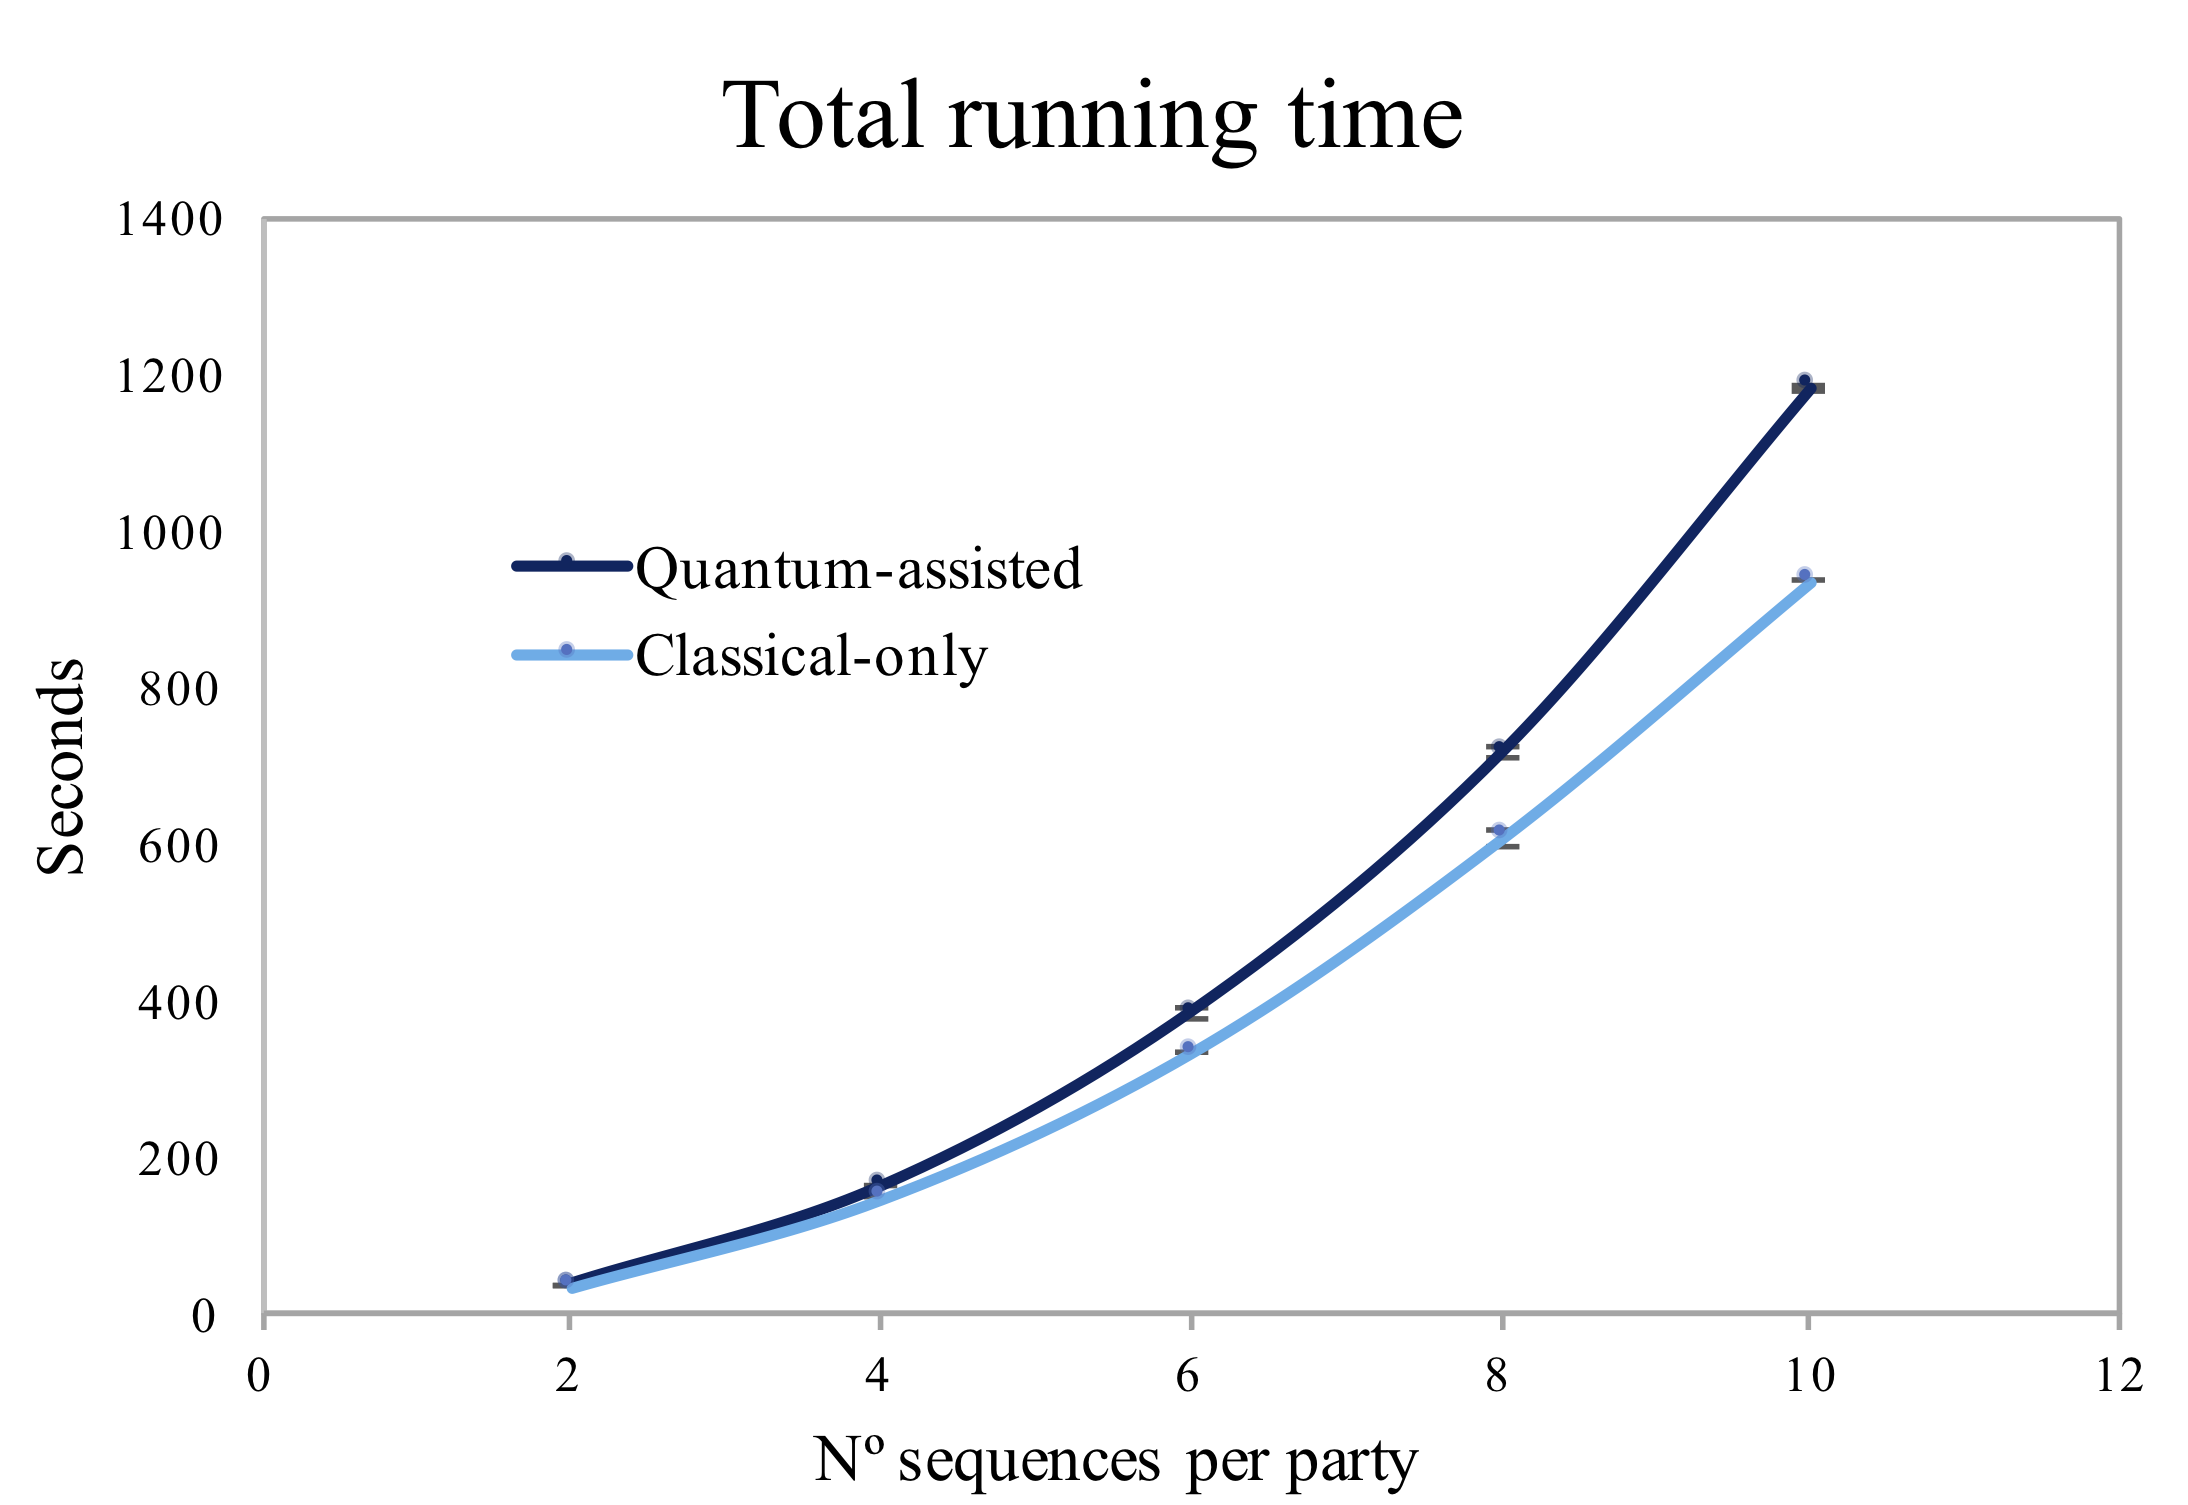
\includegraphics[scale=0.8]{Chapter_PrivatePhylogeneticTrees/total_running.png}
    \caption{Total running time of both quantum-assisted and classical-only systems.}
    \label{fig:total_running_time}
\end{figure}

Figure~\ref{fig:total_running_time} present us with the average duration of both systems with standard deviation as error bars. Here, we see that the quantum-assisted approach has a higher cost than the classical-only implementation. As discussed in section~\ref{quantumTechIntegQOT}, we can either use the $\Pi^{\textbf{BBCS}}_{\textbf{O}}$ protocol as the main OT in the Libscapi implementation or we can use it as a base OT in the KOS15 OT Extension used by Libscapi. Since we have implemented the latter, our $\Pi^{\textbf{BBCS}}_{\textbf{O}}$ is competing against the SimpleOT \cite{C15} base OT implementation. As analysed by the authors (section 4 \cite{SPM21}), the $\Pi^{\textbf{BBCS}}_{\textbf{O}}$ transfer phase is expected to outperform base OT implementations and to have comparable performance to OT Extension protocols. However, these analyses only compared cryptographic and computational operations and did not take into account implementation constraints and memory complexity.

In the quantum-assisted implementation, we separate the precomputation phase (generation of symmetric and oblivious keys) from the secure computation phase of the proposed protocol, $A^a_d$. For this reason, it is necessary to develop a key management system to save and keep key synchronization between parties. Consequently, the key management system becomes the bottleneck as the number of sequences increases. In particular, the key management system of oblivious keys is responsible for most of the overhead (Figure~\ref{fig:okms}).

\begin{figure}
    \centering
    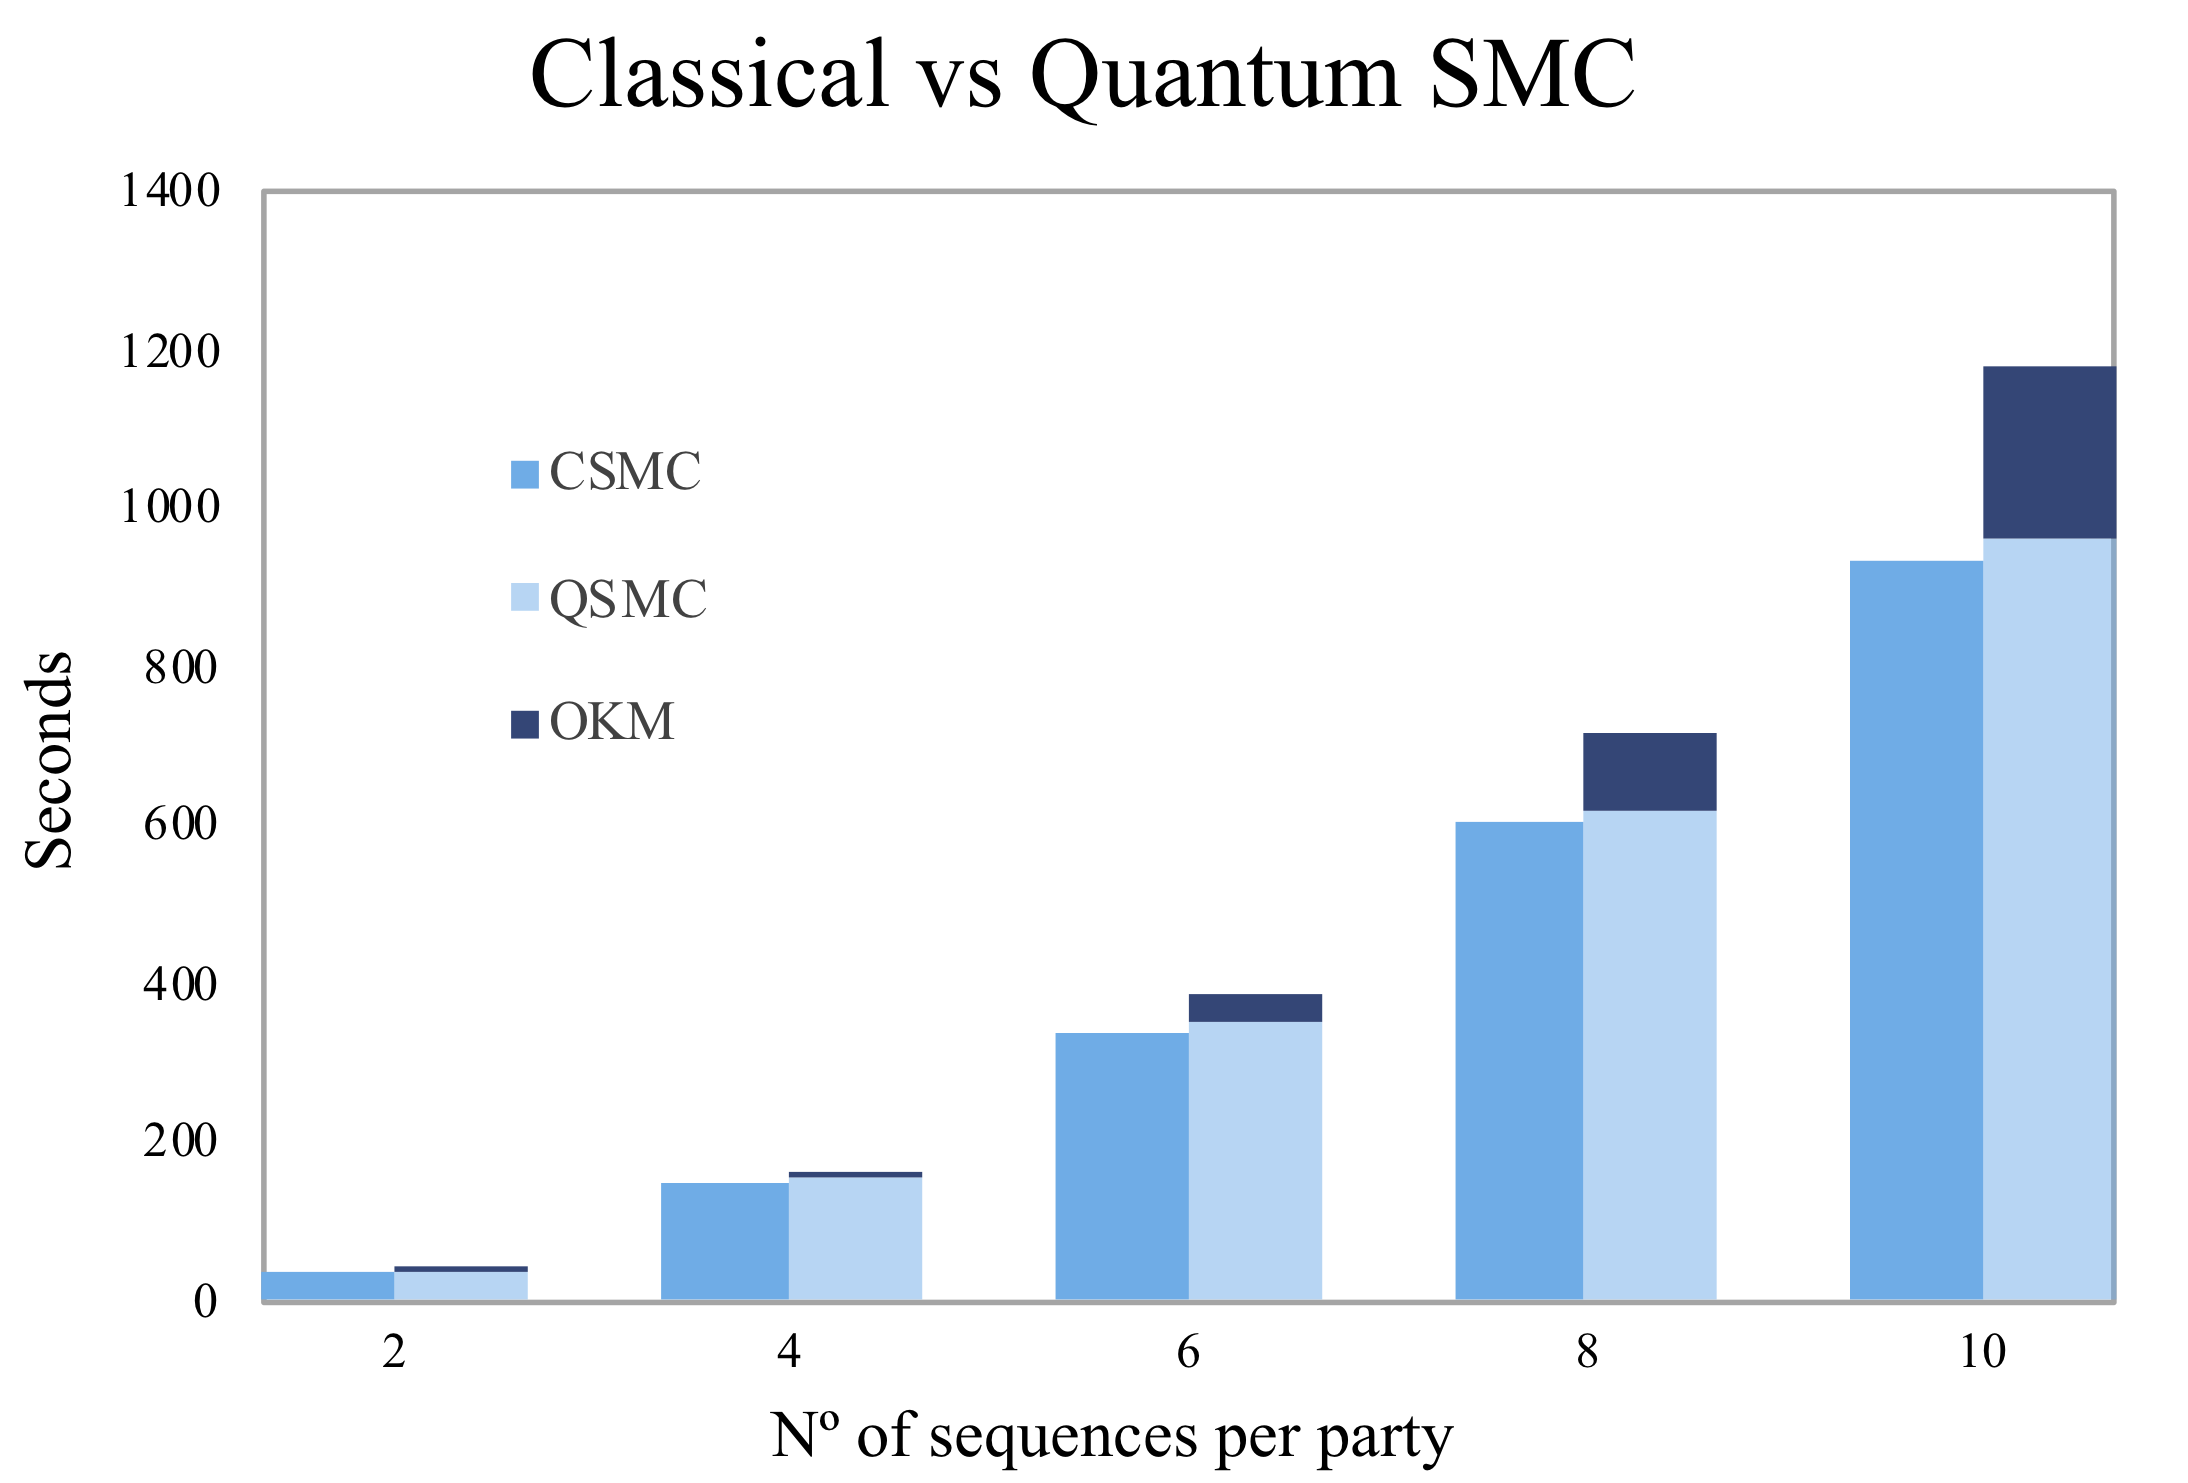
\includegraphics[scale=0.8]{Chapter_PrivatePhylogeneticTrees/c-qSMC.png}
    \caption{Total running time of the pairwise SMC computation of distances for both quantum-assisted and classical-only systems. CSMC: classical-only SMC; QSMC: quantum-assisted SMC; OKM: oblivious key management system.}
    \label{fig:okms}
\end{figure}

\begin{figure}
    \centering
    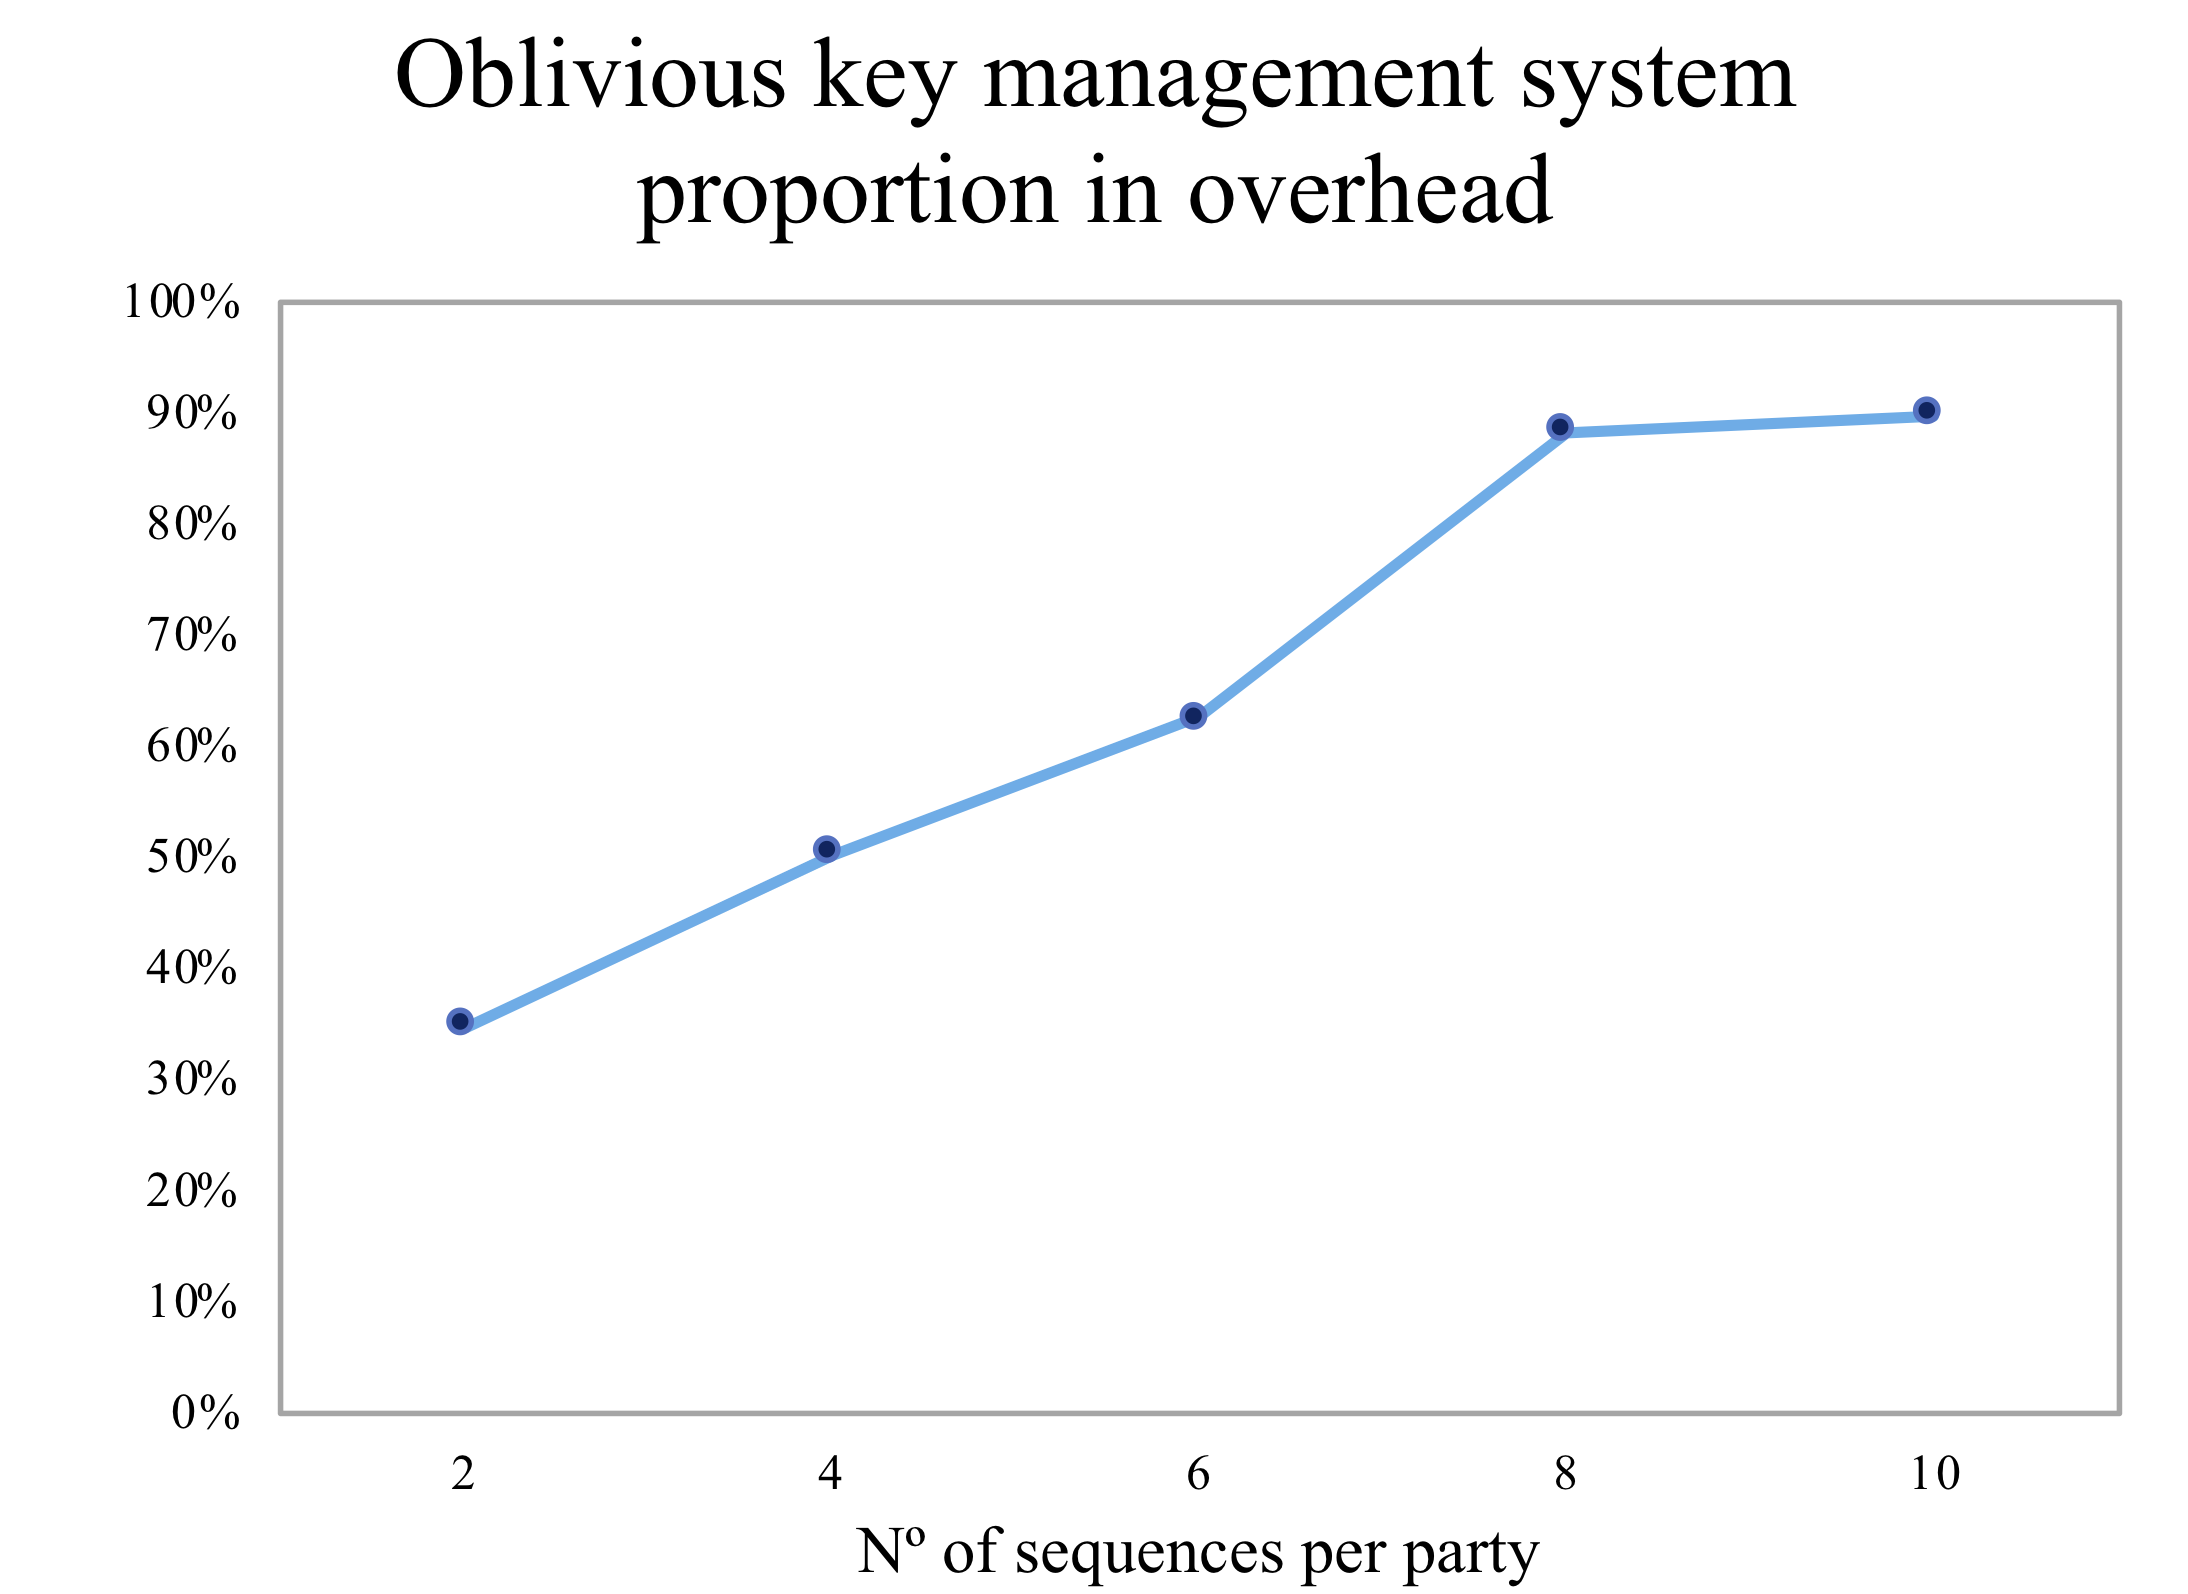
\includegraphics[scale=0.8]{Chapter_PrivatePhylogeneticTrees/proportion_in_overhead.png}
    \caption{Oblivious key management system proportion in the overhead of quantum-assisted system.}
    \label{fig:overhead}
\end{figure}

The reason for oblivious keys management to be more expensive than symmetric management and to be the main cause of overhead is twofold: the total size of oblivious keys used is three orders of magnitude higher than that of symmetric keys (compare $L^j_{qkd}$ and $L^j_{\text{bok}}$ from Table~\ref{table:complexity}); oblivious keys are loaded into ROM memory (slower access) whereas symmetric keys are loaded into RAM memory (faster access). The main reason for oblivious keys to be managed from a file system is that it allows to use Libscapi implementation of Yao protocol in a modular way, i.e. we only have to change the type of base OT used by Libscapi implementation without tailoring any other module.

As the management of files is time-sensitive to their size, the proportion of time spent on the overhead due to the oblivious key management system (OKM) increases with the number of shared keys per party. This can be confirmed by Figure~\ref{fig:overhead} which shows the proportion of time spent by the oblivious key management system in the difference between the quantum-assisted and the classical-only system.

Future work is required to develop more efficient oblivious key management systems. Despite this difference, we stress that the quantum-assisted system has a significantly higher degree of security against quantum computer attacks.

%However, a key management system is only needed in case we separate the oblivious key generation from the online secure computation. In Table~\ref{table:complexity} we estimated the time to generate . Nevertheless, this implementation choice depends on the best scenario  \hl{ Para além de melhorar o okm: Comentar a opção de fazer logo tudo e não precisar de um key management system. Para valores correntes pode se fazer isso e o tempo de geração (segundo os valores estimados) outperform o overhead dado pelo OKM - comparar resultados para o caso.}



\section{Conclusion}

In this chapter, we presented an SMC protocol assisted with quantum technologies tailored for distance-based algorithms of phylogenetic trees. It is a modular protocol that uses one distance metric taken from four possible evolutionary models (Jukes-Cantor, Kimura 2-parameter, F84 and LogDet) and three different protocols (UPGMA, Neighbour-Joining and Fitch-Margoliash). In total, we can implement twelve different combinations of protocols.

The proposed system is based on ready to use libraries (CBMC-GC, Libscapi and PHYLIP) that are integrated with quantum technologies to provide a full quantum-proof solution. We use the quantum version of primitives that play a central role in the security of the system: oblivious transfer, encryption and random number generation.

We compare the performance of a classical-only and a quantum-assisted system based on simulated symmetric and oblivious keys. Previous analyses on the computation and communication complexity point to a scenario where the quantum-assisted version does not add an extra efficiency cost. This is confirmed by comparing the running times of both approaches without considering the overhead created by the oblivious key management system that increases with the number of shared keys. Further work is required to develop more efficient key management systems. Despite this extra cost, the quantum-assisted version significantly improves the system security when compared with the classical-only as it renders a protocol with enhanced security against quantum computers.








%\bibliography{bibforthesis}
%\bibliographystyle{unsrt}
%\end{document}
